\section{Corrections to simulation}
\label{corrections}

We apply several corrections to the simulated background and signal events in order to account for known differences between simulation and data. Each correction is described individually in the following sections.

\subsection{Event pileup}
The  simulation is corrected so that its distribution of the number of pileup interactions matches that of 2016, 2017, and 2018 data. Each simulated sample is reweighted, event-by-event, by scale factors derived by dividing the pileup distribution in data by the pileup distribution in the given simulated sample.\fxnote{add plots?}

\subsection{Lepton ID}
We apply scale factors provided by the CMS Physics Object Groups to correct for known differences in the lepton reconstruction and tight ID performance between data and simulation. Although our lepton ID differs from the standard tight ID in that we do not set requirements on \ad or the longitudinal impact parameter, the standard scale factors are still sufficient because they are derived from leptons from $\cPZ$ boson decays that are representative of leptons in the bulk of the \ad distribution, and we apply additional systematic uncertainties to account for possible differences at larger \ad (see Section~\ref{systematics}).

\subsection{Lepton $d_0$ resolution}\fxnote{move details to appendix?}
\label{d0_smearing}
As shown in Fig.~\ref{uncorrected_d0}, the agreement between data and simulation in the 2017 and 2018 electron and muon \ad distributions was initially poor. We found that the average muon and electron $d_0$ fluctuated periodically with respect to $\phi$ in 2017 and 2018 data but not in background simulation, as can be seen in Fig.~\ref{uncorrected_avg_d0_vs_phi}. This periodic fluctuation in data but not in simulation indicates that an overly optimistic simulated tracker alignment is responsible for the unrealistically narrow $d_0$ distribution in simulation.

\begin{figure}
\centering
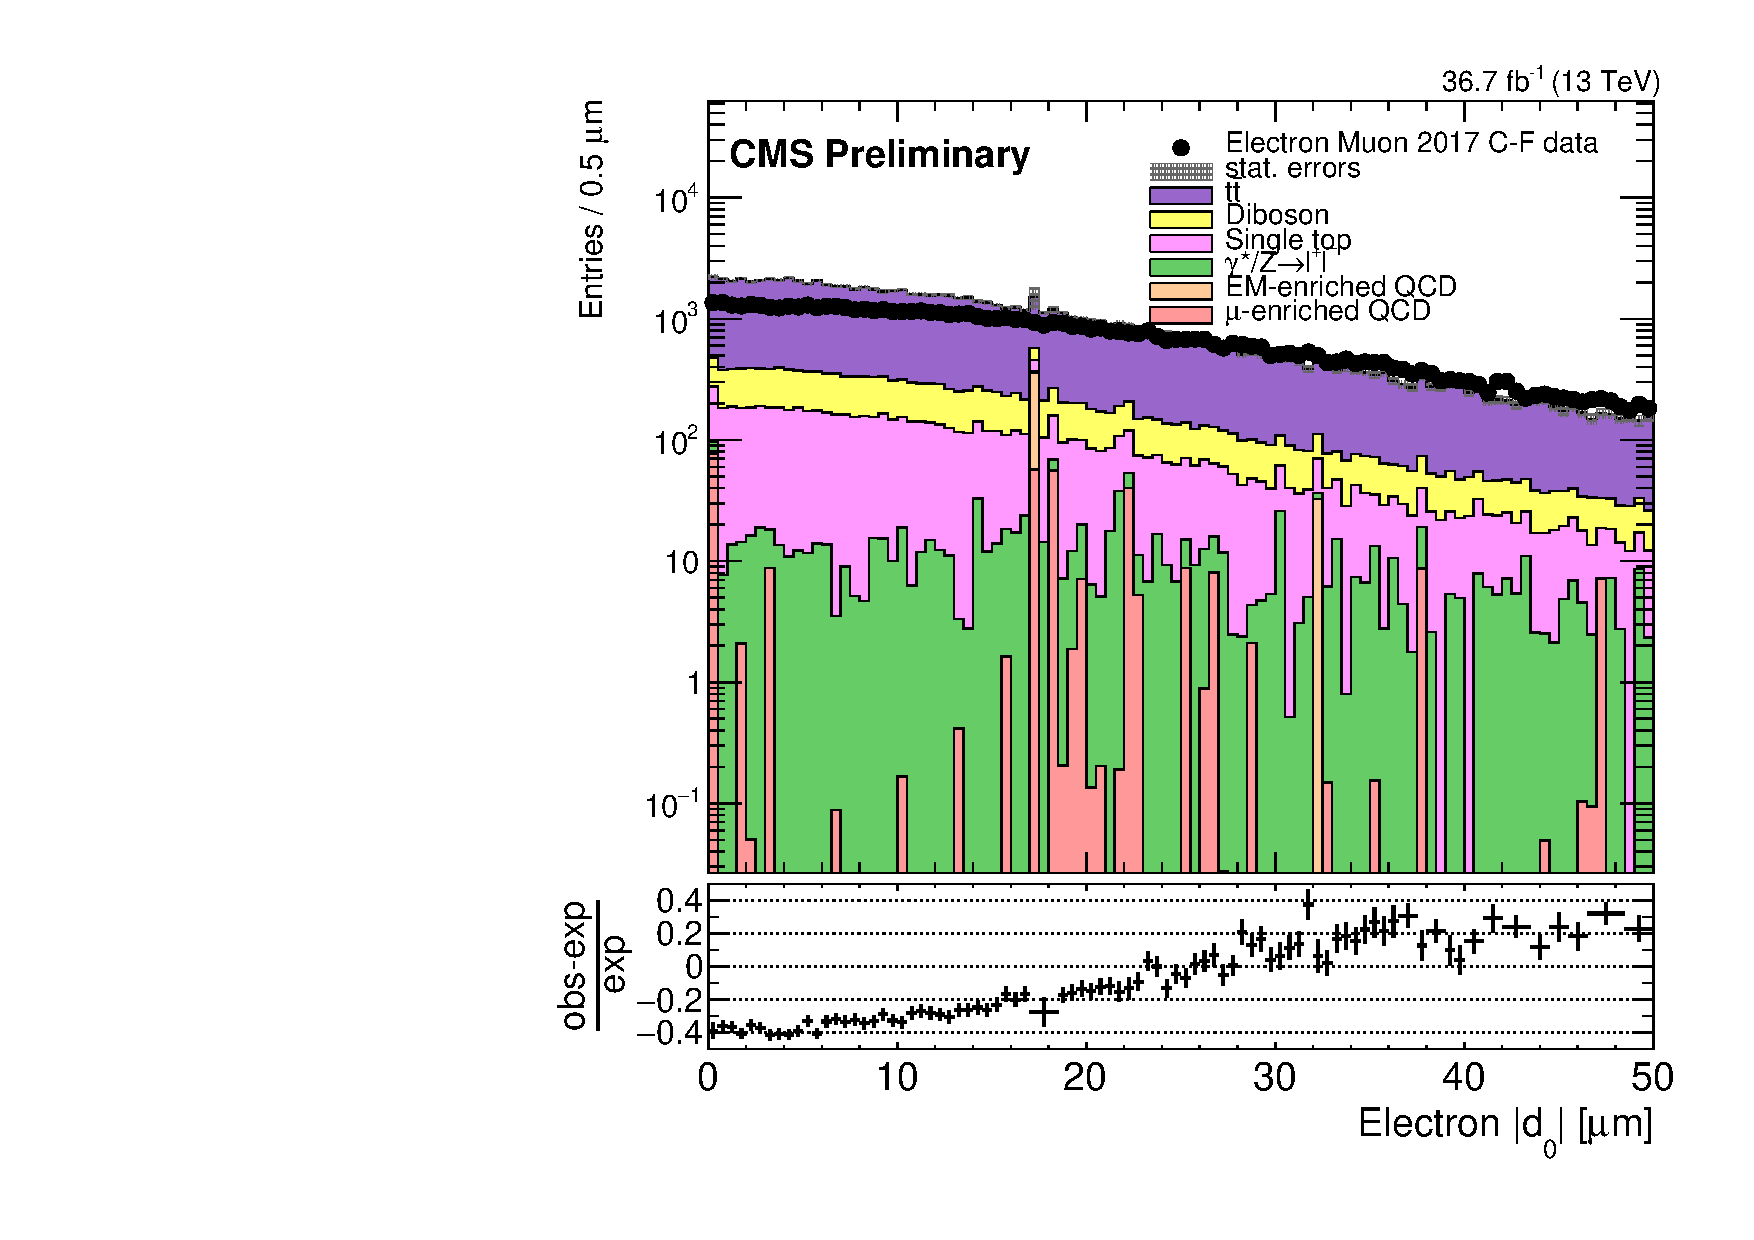
\includegraphics[width=0.4\textwidth]{figures/corrections/d0_smearing/emu_2017/electronAbsD0_50um_uncorrected.pdf} 
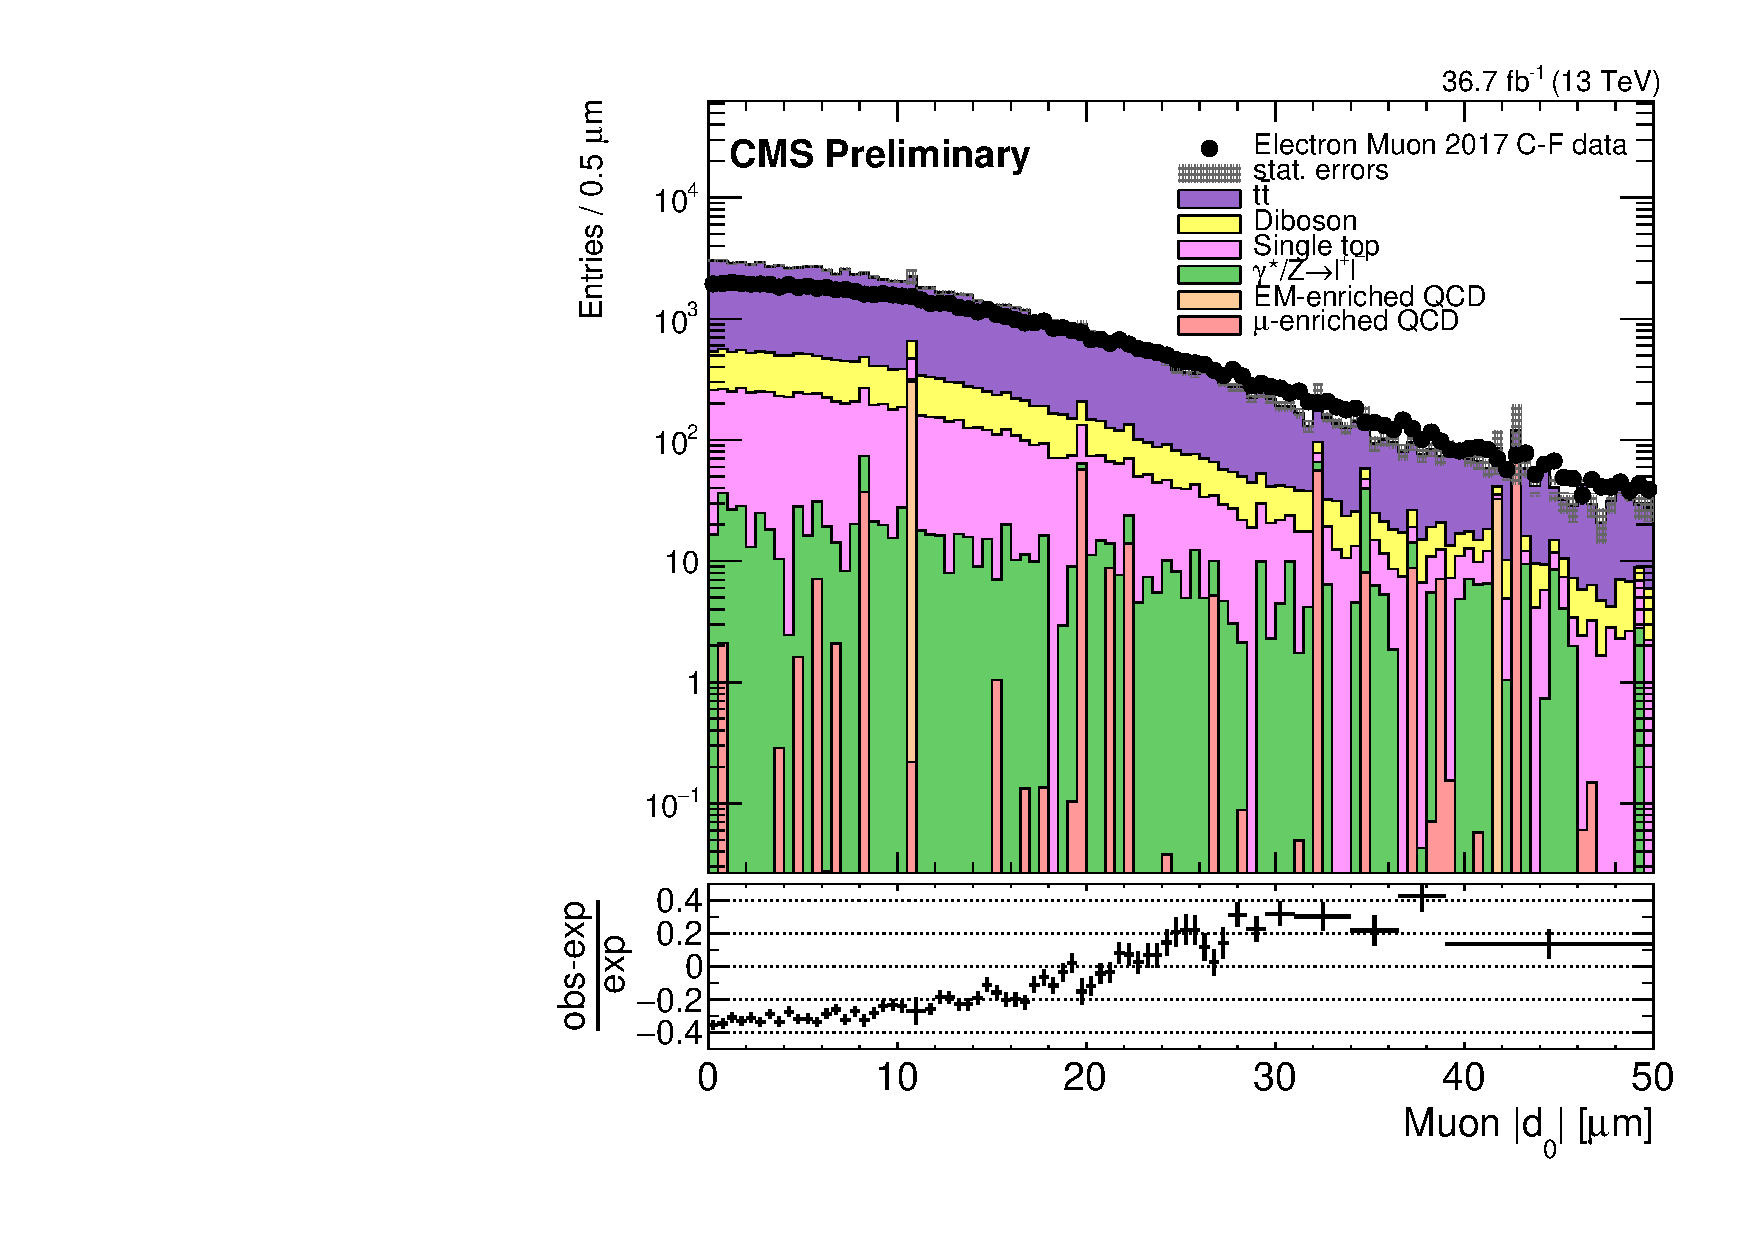
\includegraphics[width=0.4\textwidth]{figures/corrections/d0_smearing/emu_2017/muonAbsD0_50um_uncorrected.pdf}
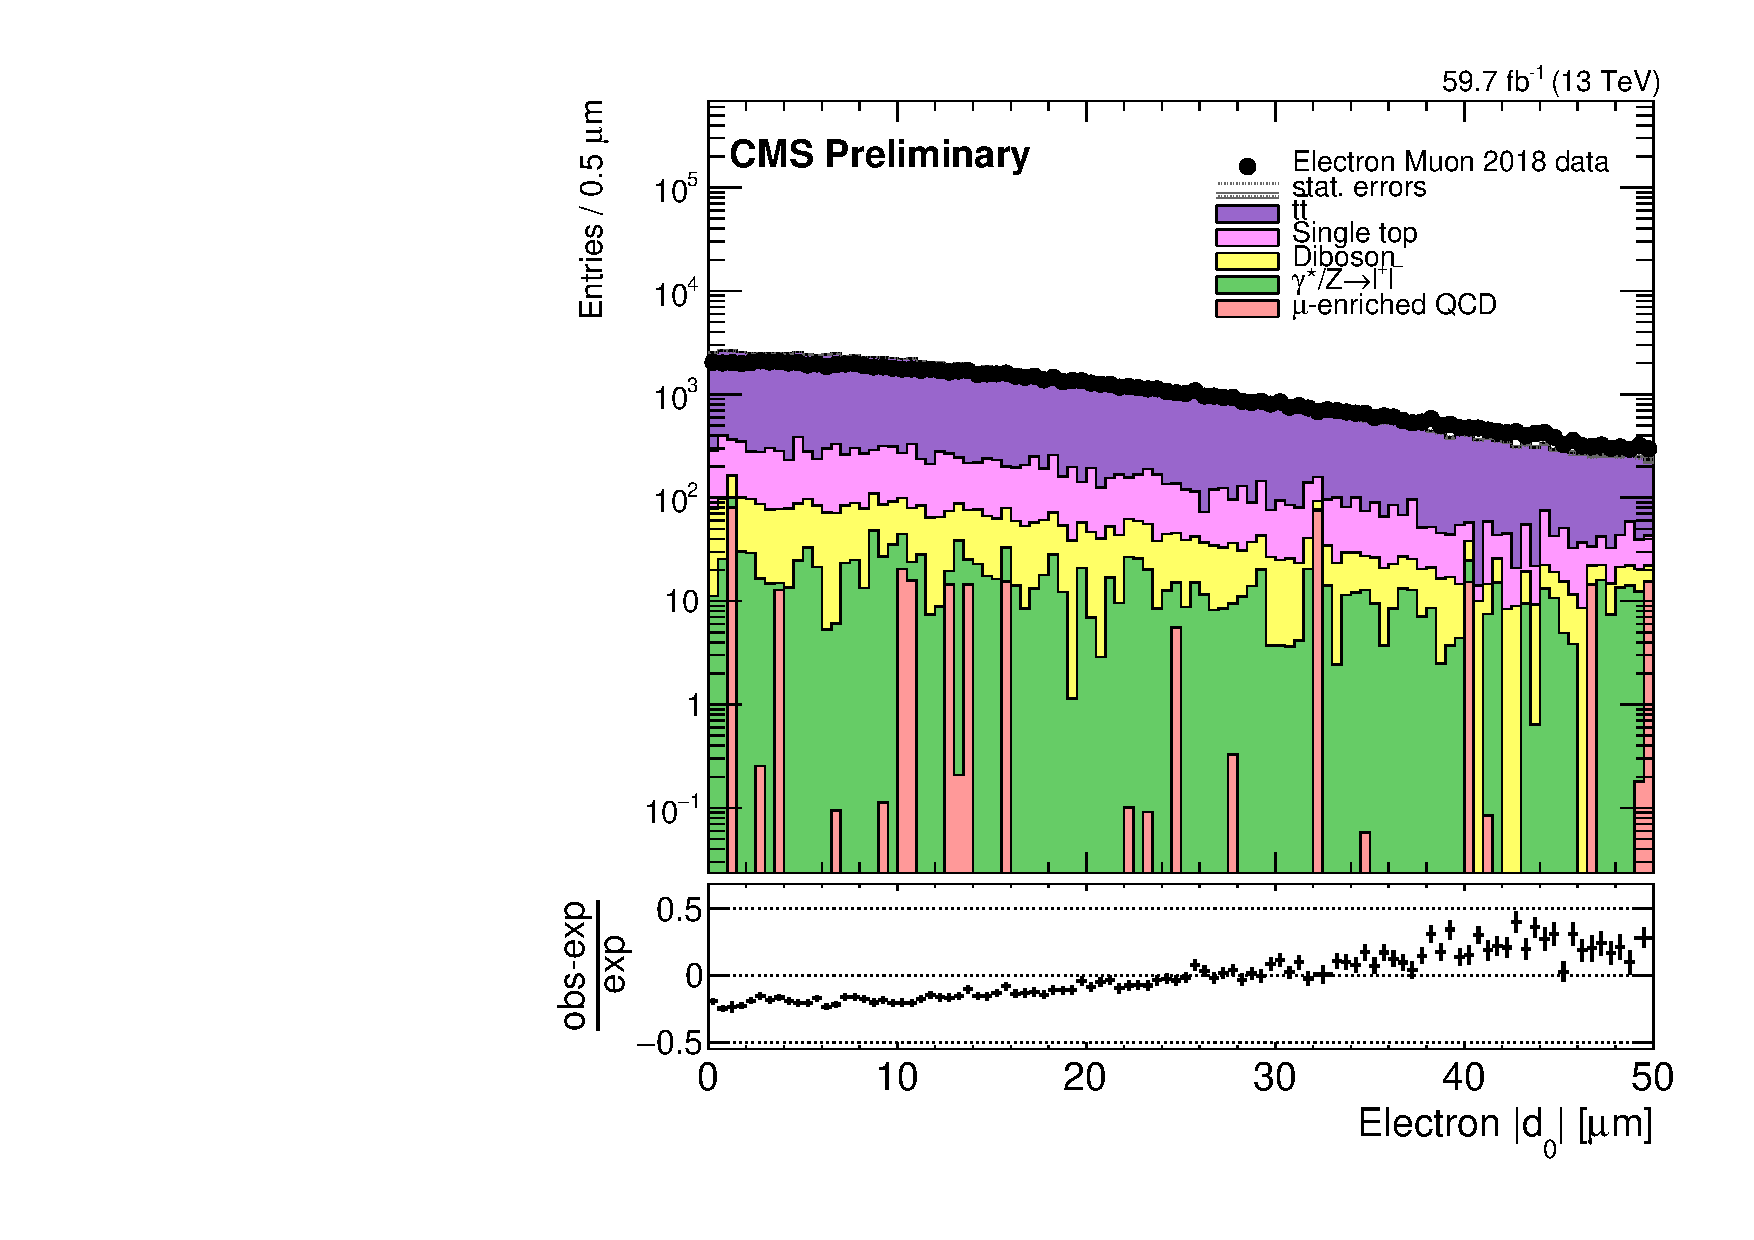
\includegraphics[width=0.4\textwidth]{figures/corrections/d0_smearing/emu_2018/electronAbsD0_50um_uncorrected.pdf} 
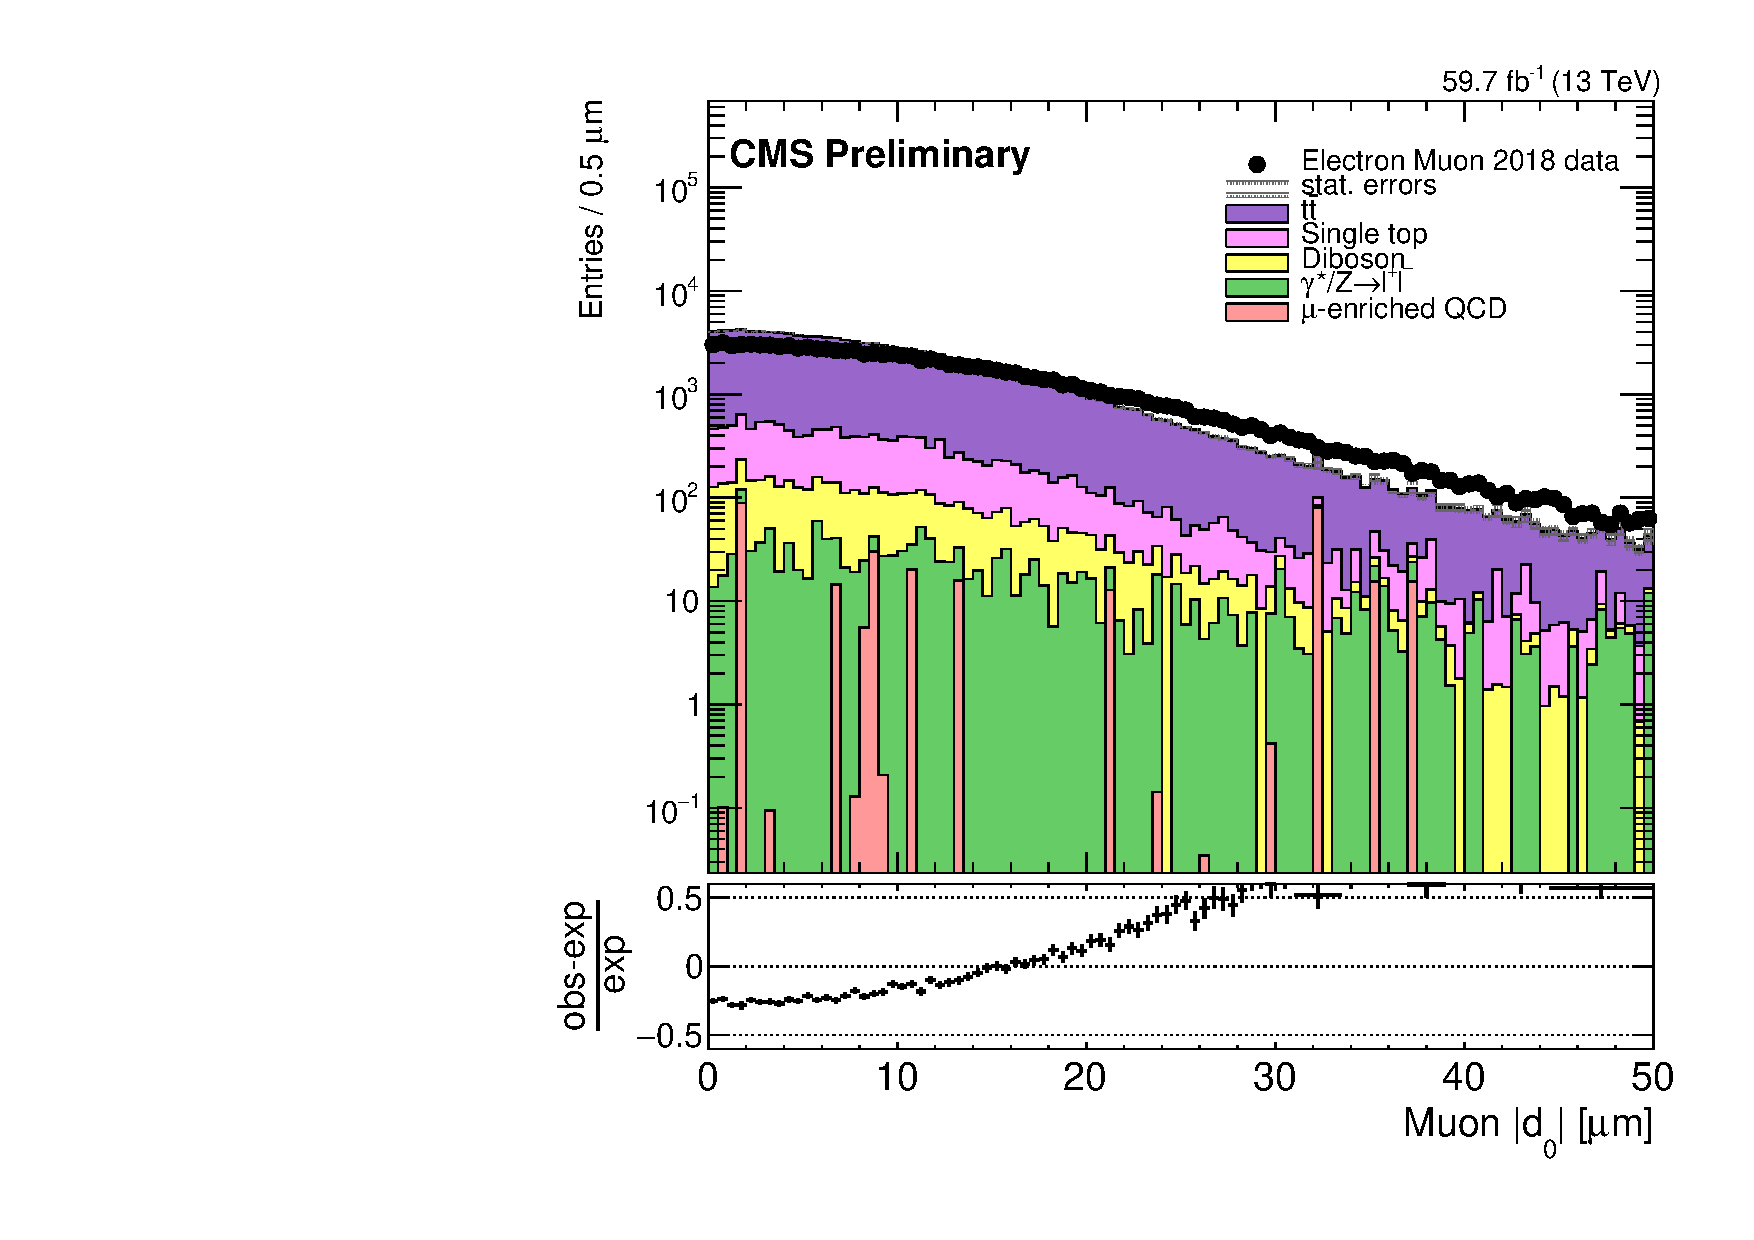
\includegraphics[width=0.4\textwidth]{figures/corrections/d0_smearing/emu_2018/muonAbsD0_50um_uncorrected.pdf}
\caption{The uncorrected lepton \ad distributions in the $\Pe\Pgm$ prompt control region, for electrons (left) and muons (right), for 2017 data and simulation (upper), and 2018 data and simulation (lower). The rightmost bin in each plot
contains the overflow entries.}
\label{uncorrected_d0}
\end{figure}

To account for the overly optimistic alignment in simulation, we smear the electron and muon $d_0$ in 2017 and 2018 simulation in each channel's prompt control region to better model the $d_0$ distribution in data. To do this, we first fit the central regions of the background simulation and data $d_0$ distributions with Gaussian functions in each channel's prompt control region and then compare the widths of the Gaussian fits. The fitted distributions are shown in Figs.~\ref{gaussian_fits_2017} and \ref{gaussian_fits_2018} for the $\Pe\Pgm$ channel. Assuming that the width of each Gaussian fit is mostly determined by the $d_0$ resolution, we define $\sigma_{data}^2 = \sigma_{bkg}^2 + \sigma_{align}^2$, where $\sigma_{data}$ is the data Gaussian width, $\sigma_{bkd}$ is the uncorrected background simulation Gaussian width, and $\sigma_{align}$ is the additional component that is needed to make up the difference in $d_0$ resolution between background simulation and data. We find $\sigma_{data}$ and $\sigma_{bkg}$ from the fits and compute $\sigma_{align}$. The fit results are similar in the $\Pe\Pgm$ channel shown here and in the same-flavor channels. We average the $\sigma_{align}$ derived in the $\Pe\Pe$ channel and the $\Pe\Pgm$ channel for electrons, and in the $\Pgm\Pgm$ channel and the $\Pe\Pgm$ channel for muons. The average $\sigma_{align}$ is shown in Table~\ref{sigma_align}. We then smear the simulation $d_0$ values with values drawn from a Gaussian distribution centered on zero and with a width of the average $\sigma_{align}$. The smearing is applied to both background and signal simulation. The corrected \ad distributions are shown in Fig.~\ref{corrected_d0}.

\begin{figure}[hbtp]
\centering
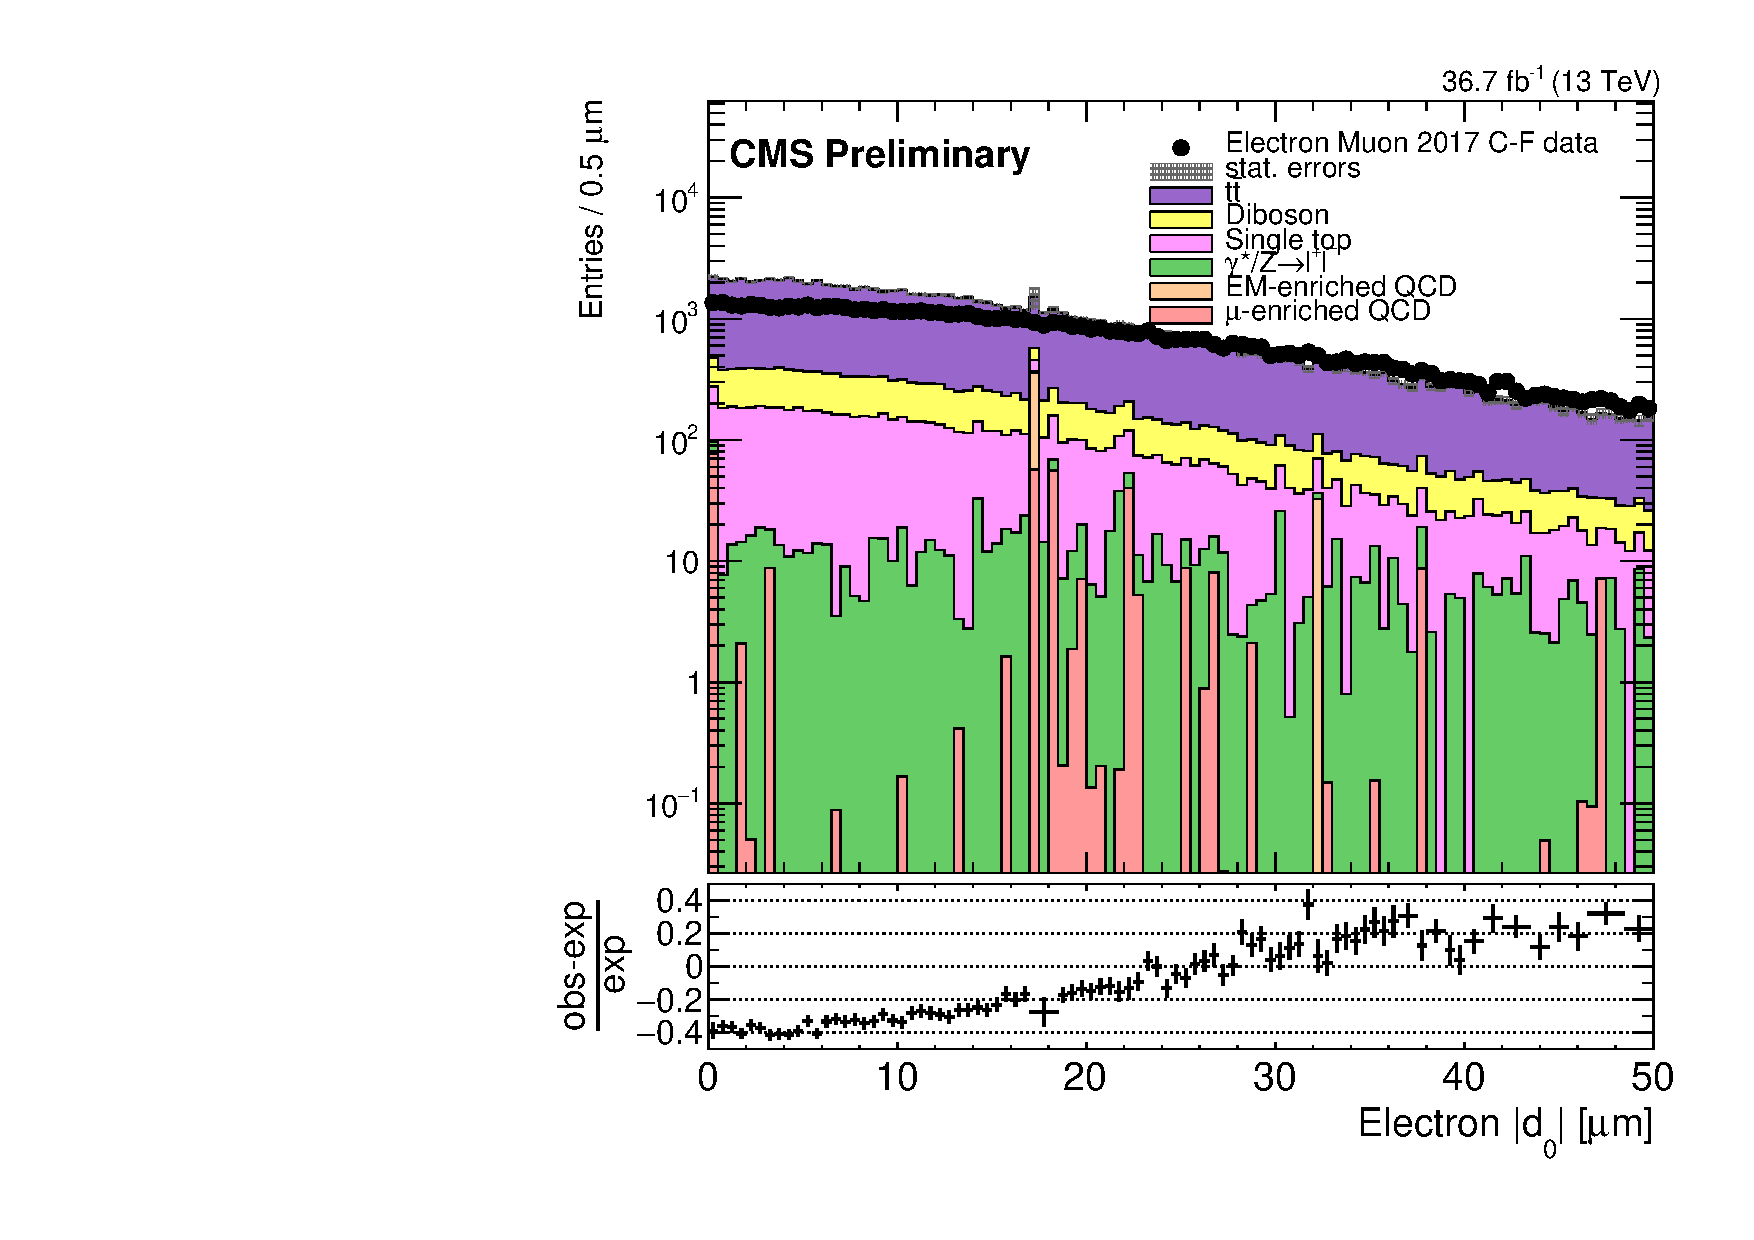
\includegraphics[scale=0.3]{figures/corrections/d0_smearing/emu_2017/electronAbsD0_50um_uncorrected.pdf} 
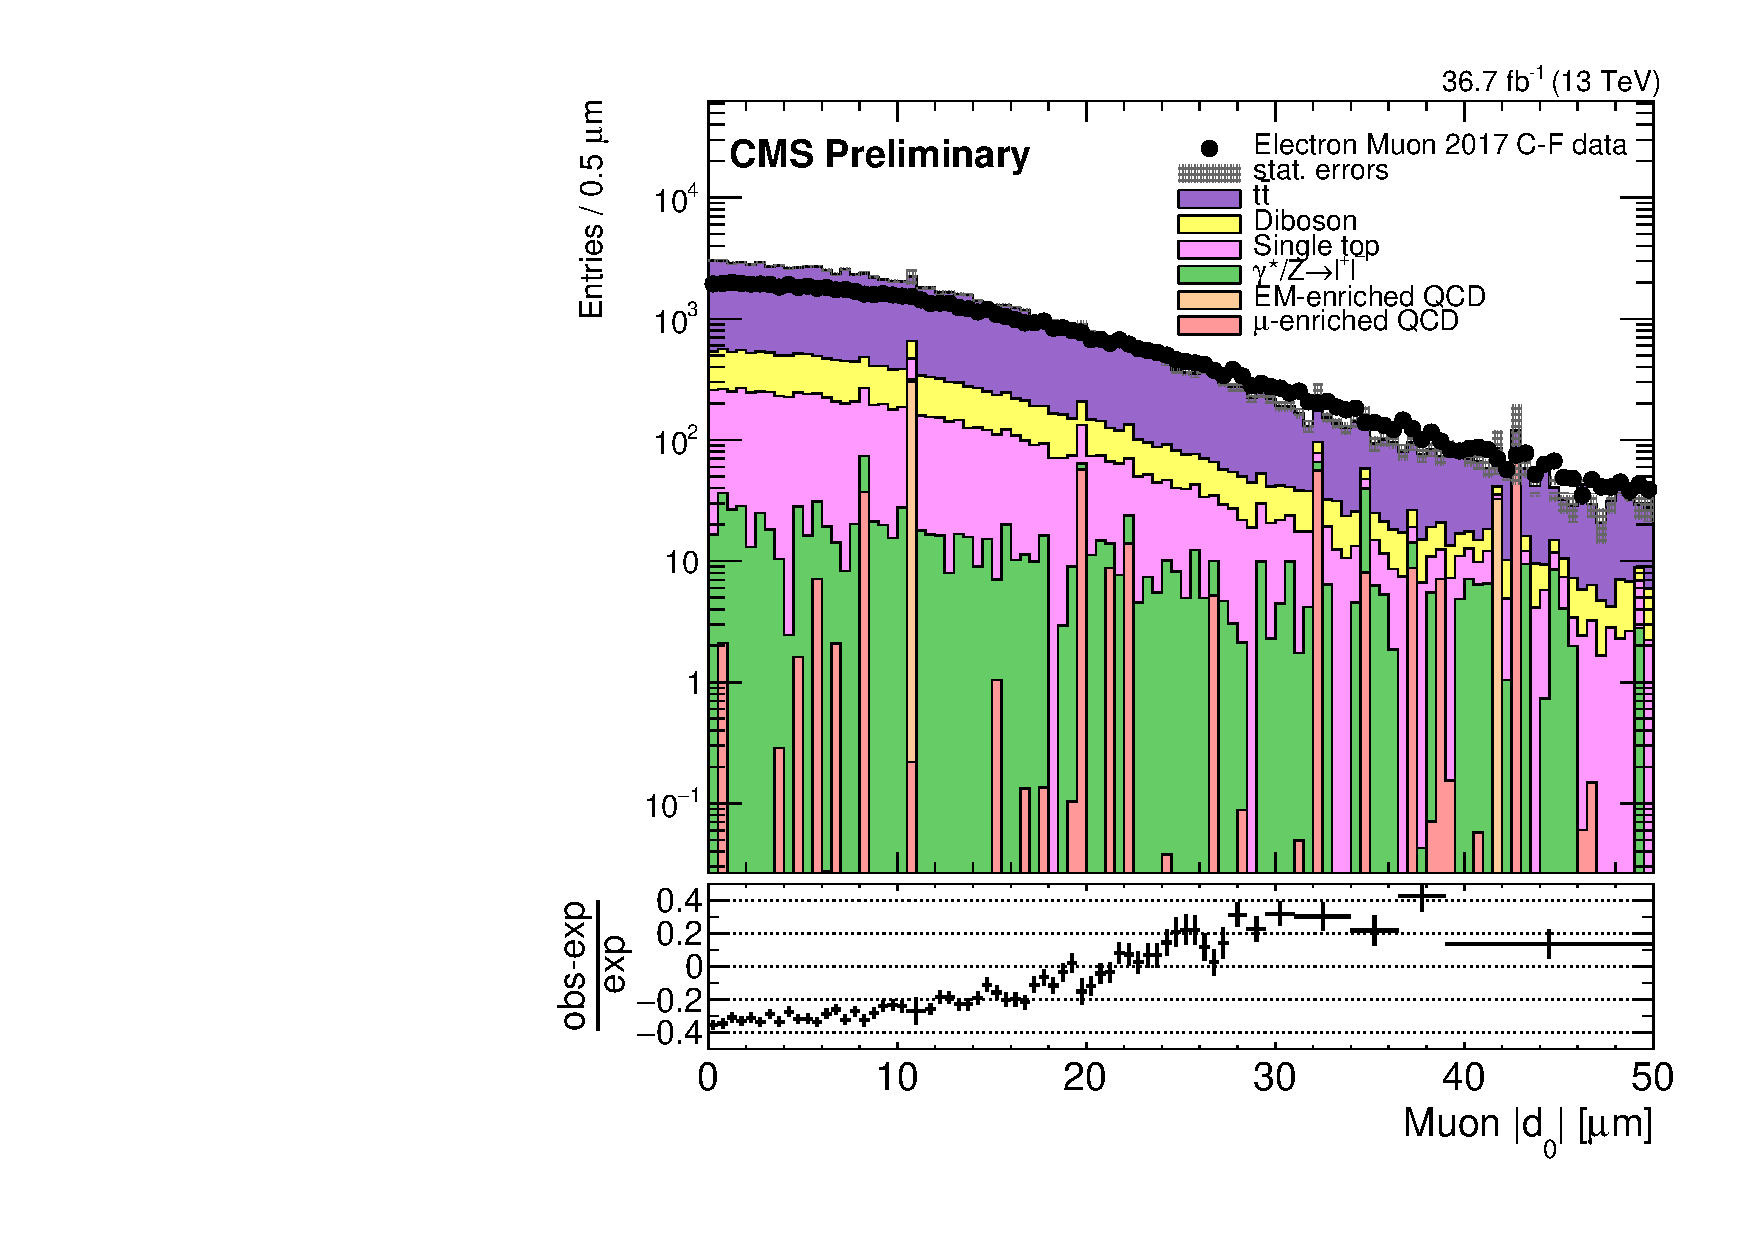
\includegraphics[scale=0.3]{figures/corrections/d0_smearing/emu_2017/muonAbsD0_50um_uncorrected.pdf}
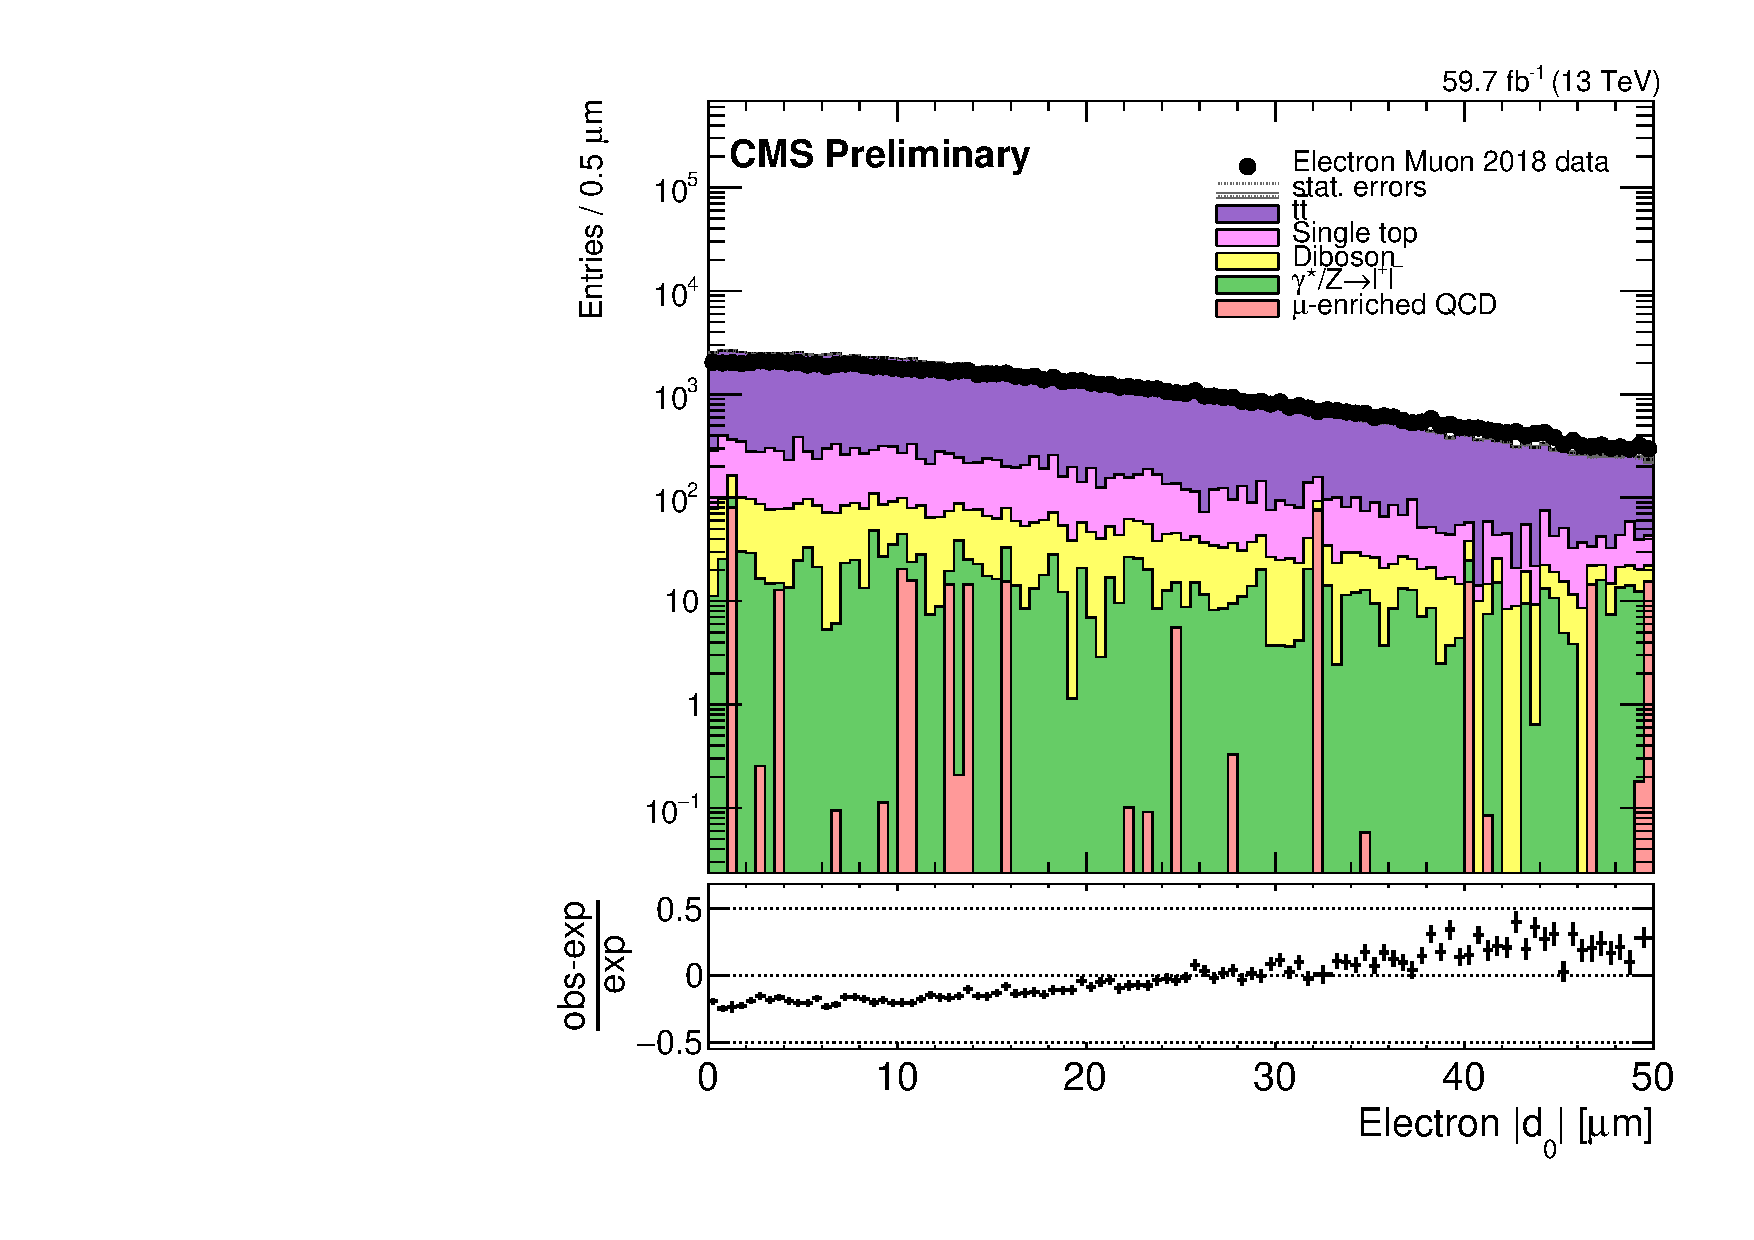
\includegraphics[scale=0.3]{figures/corrections/d0_smearing/emu_2018/electronAbsD0_50um_uncorrected.pdf} 
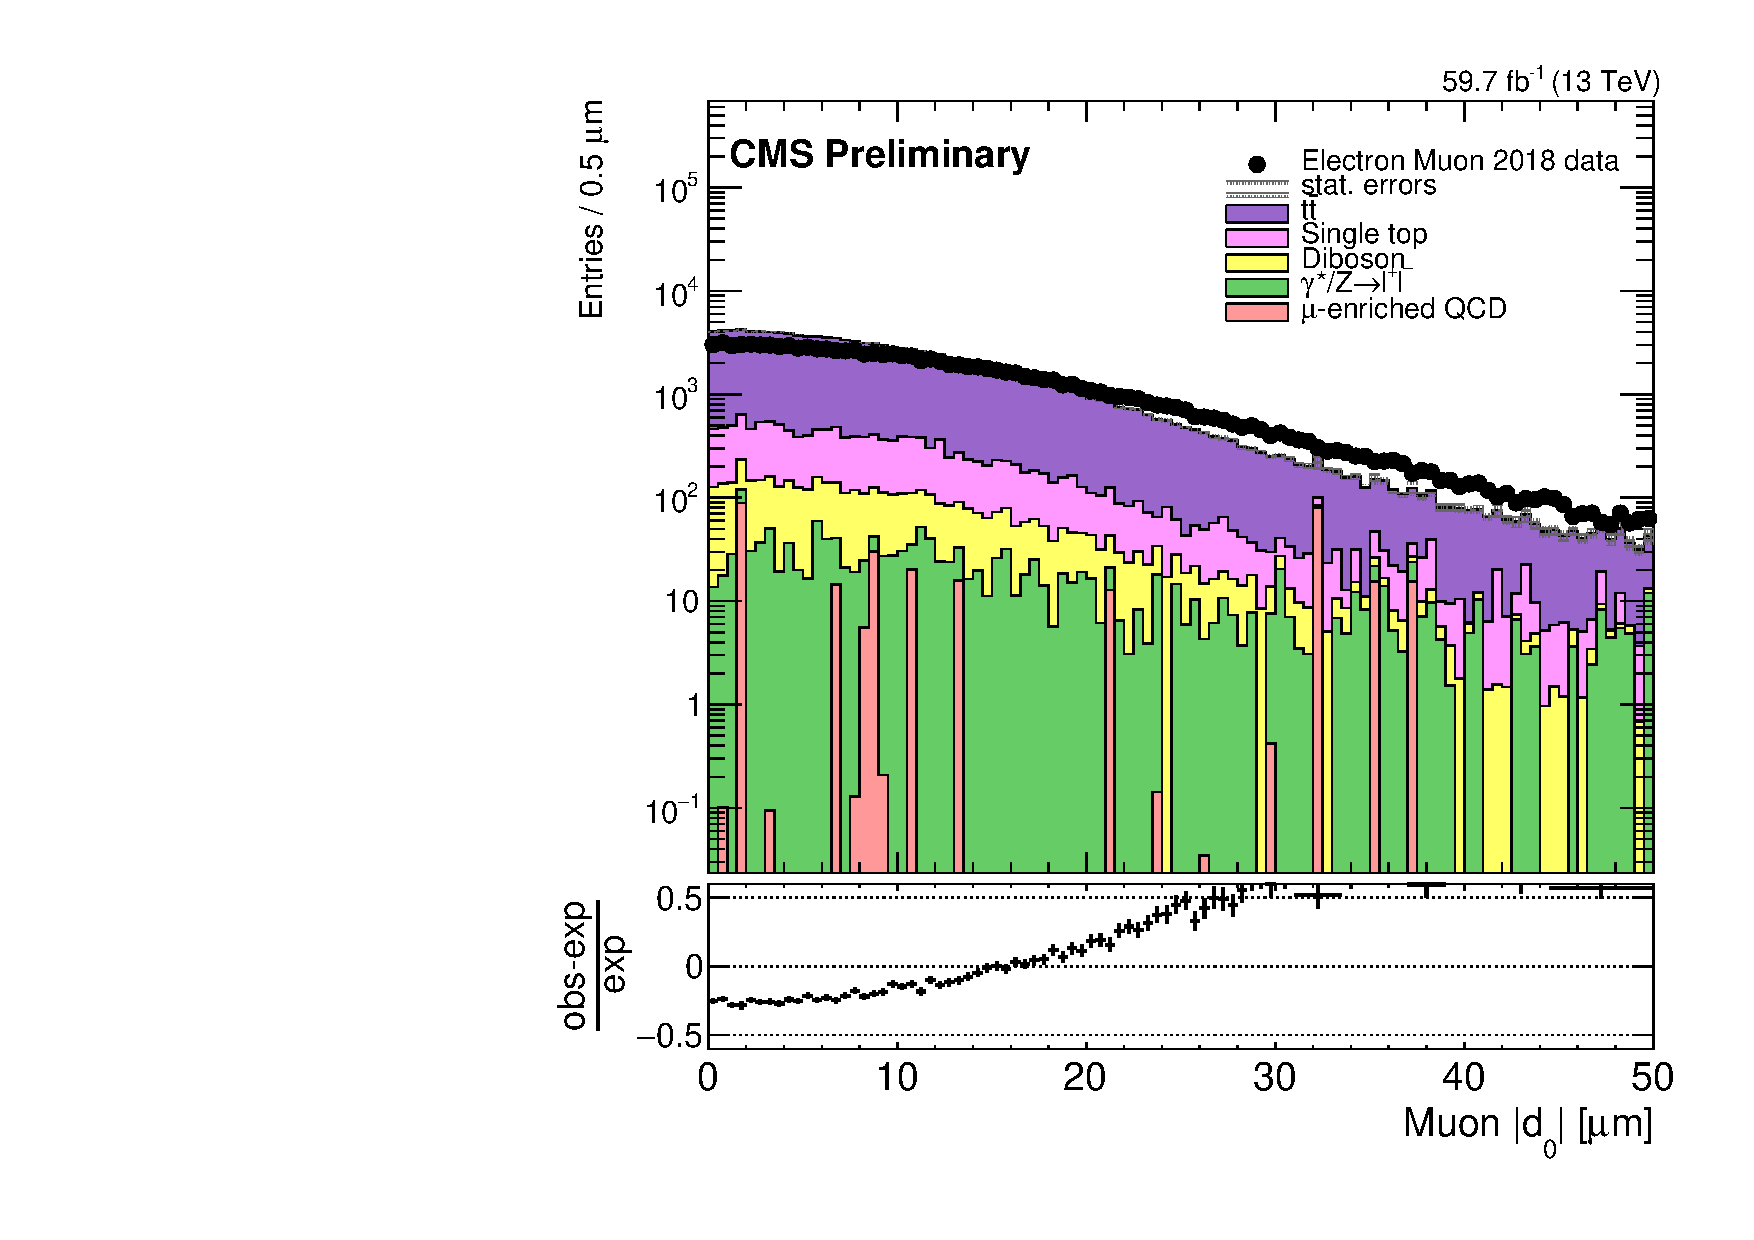
\includegraphics[scale=0.3]{figures/corrections/d0_smearing/emu_2018/muonAbsD0_50um_uncorrected.pdf}
\caption{The uncorrected lepton \ad distributions in the $\Pe\Pgm$ prompt control region, for electrons (left) and muons (right), for 2017 data and simulation (upper), and 2018 data and simulation (lower). The rightmost bin in each plot
contains the overflow entries.}
\label{uncorrected_d0}
\end{figure}

\begin{figure}[hbtp]
\centering
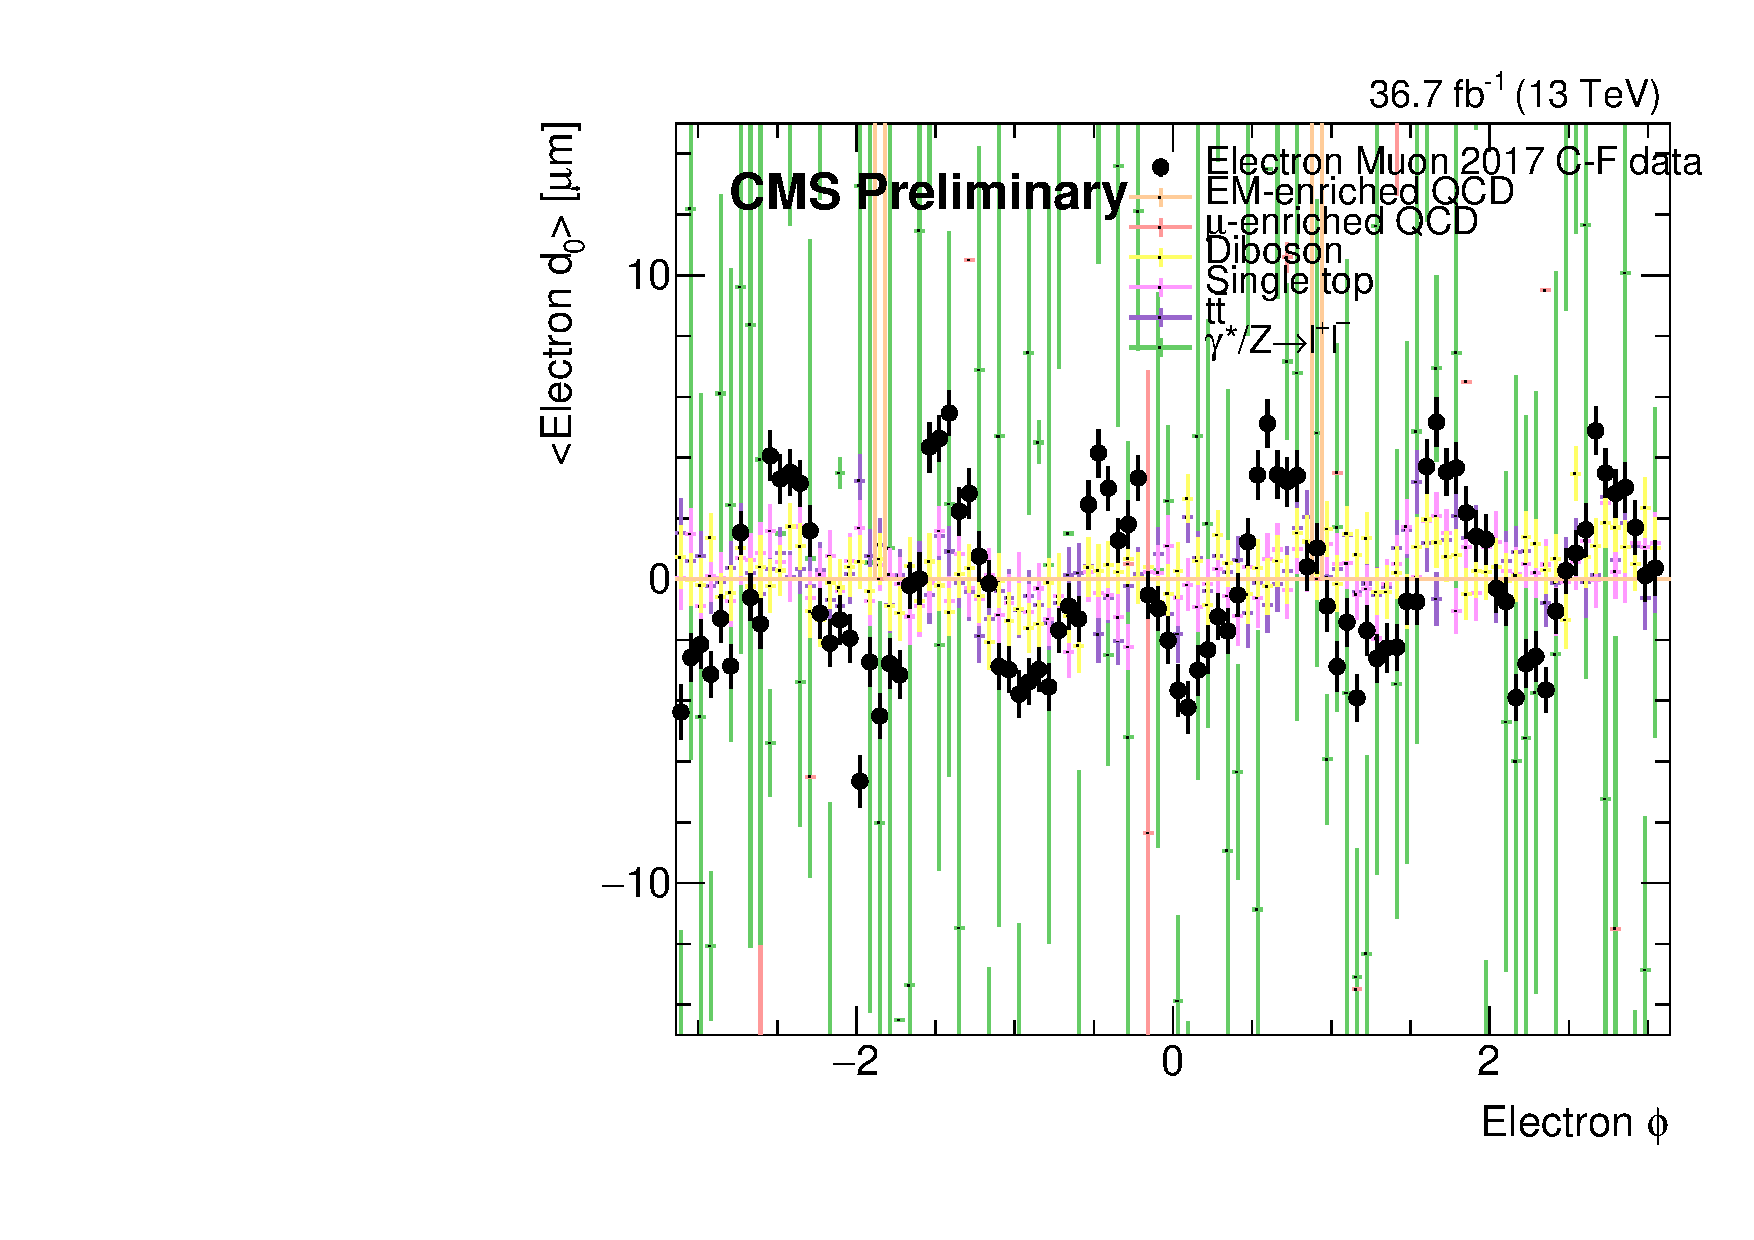
\includegraphics[scale=0.3]{figures/corrections/d0_smearing/emu_2017/electronD0_50um_vs_electronPhi_pfx.pdf}
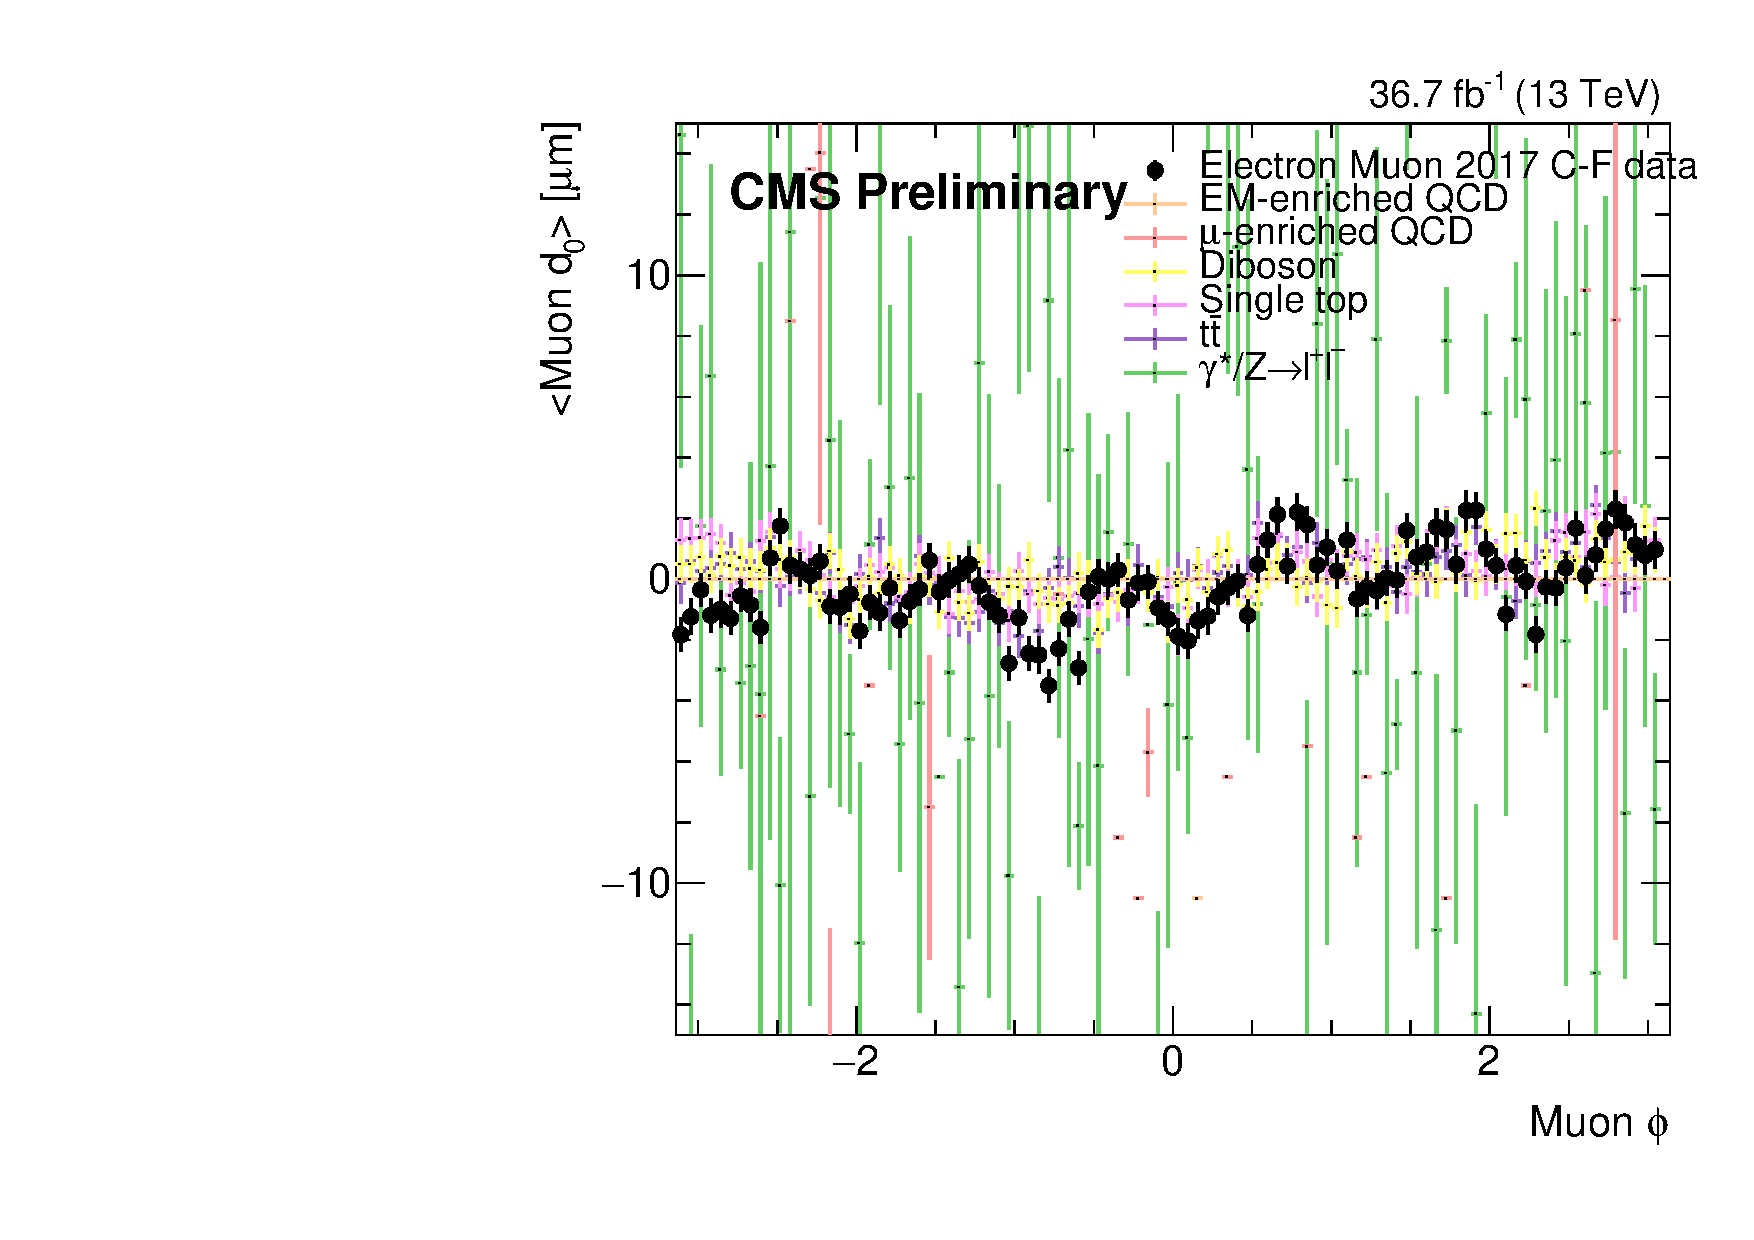
\includegraphics[scale=0.3]{figures/corrections/d0_smearing/emu_2017/muonD0_50um_vs_muonPhi_pfx.pdf}
\caption{The average lepton \ad as a function of $\phi$ in the $\Pe\Pgm$ prompt control region, for electrons (left) and muons (right), for 2017 data and simulation.}
\label{uncorrected_avg_d0_vs_phi}
\end{figure}

\begin{figure}[hbtp]
\centering
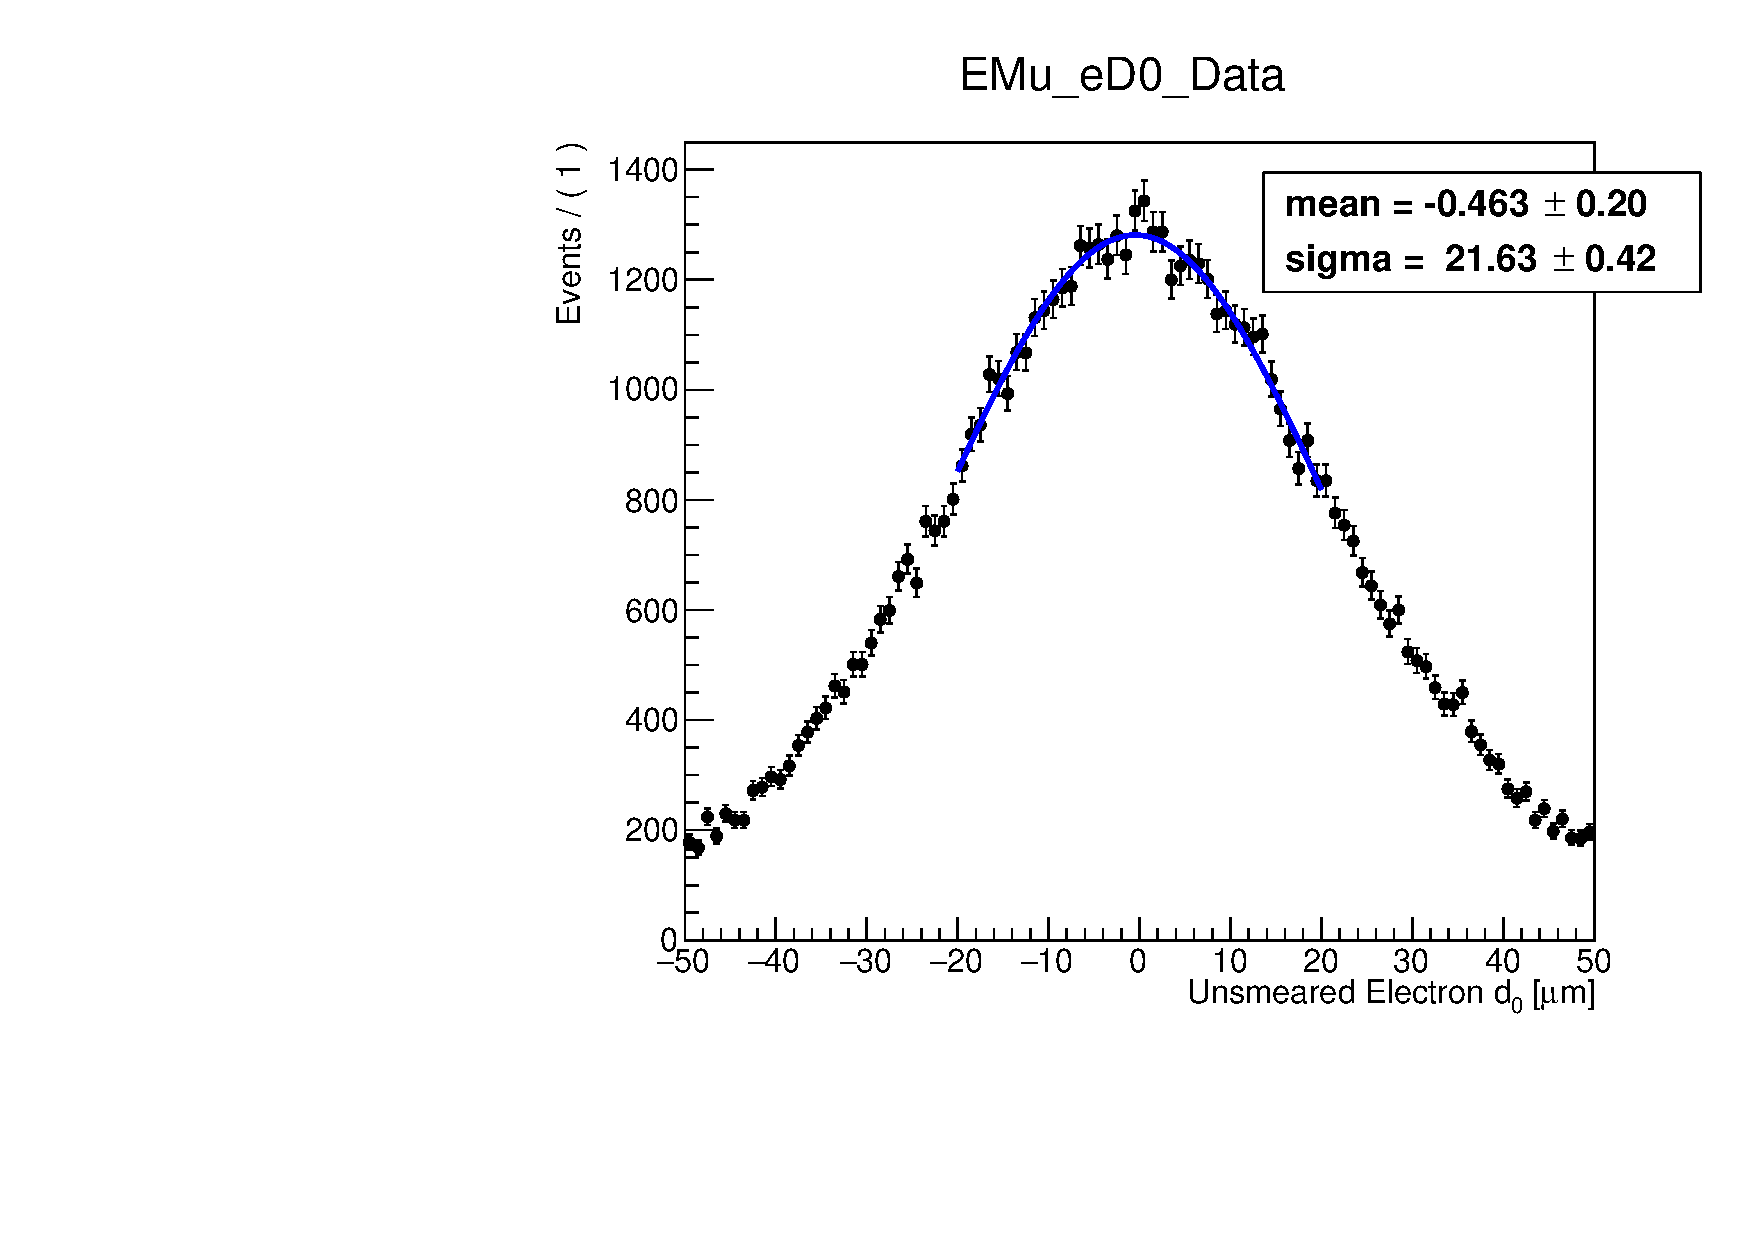
\includegraphics[scale=0.3]{figures/corrections/d0_smearing/emu_2017/gaussian_fit_EMu_eD0_Data.pdf}
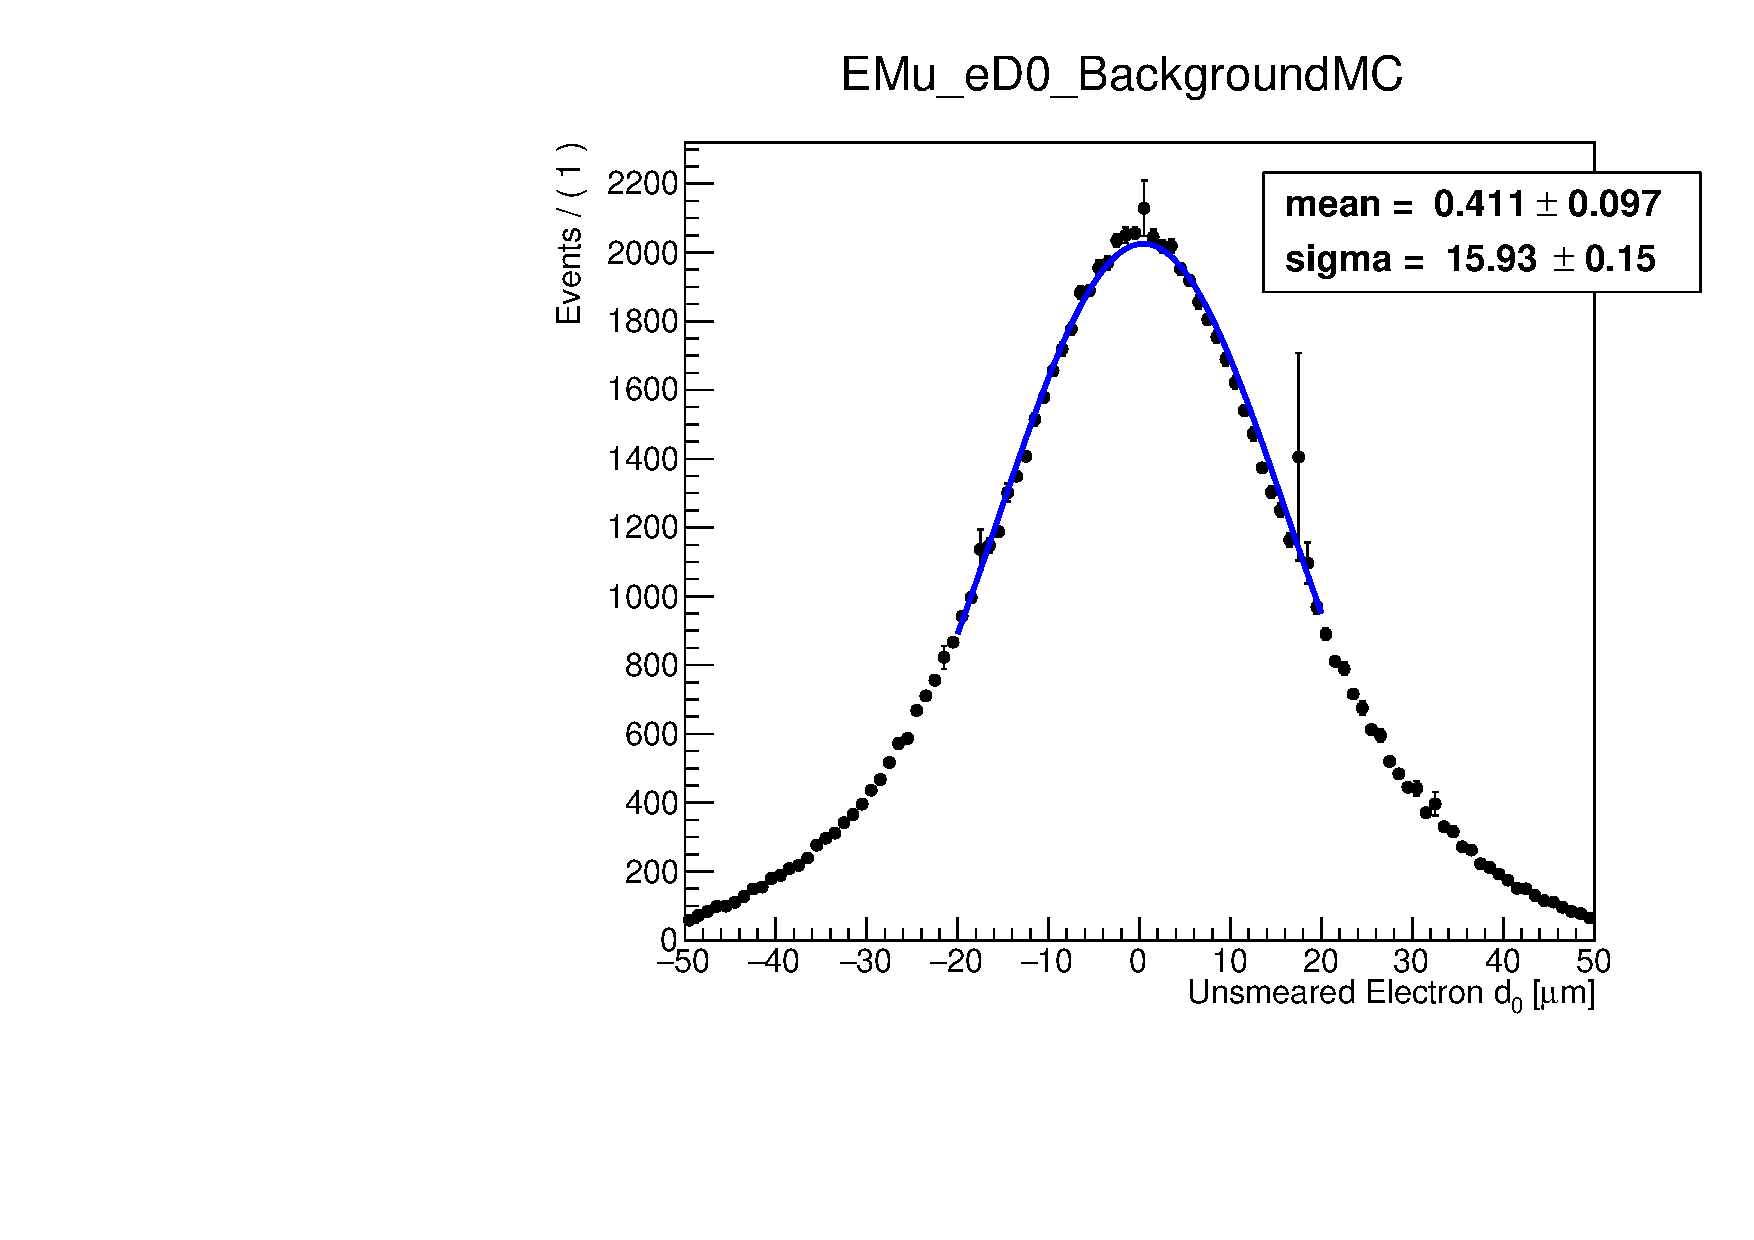
\includegraphics[scale=0.3]{figures/corrections/d0_smearing/emu_2017/gaussian_fit_EMu_eD0_BackgroundMC.pdf}
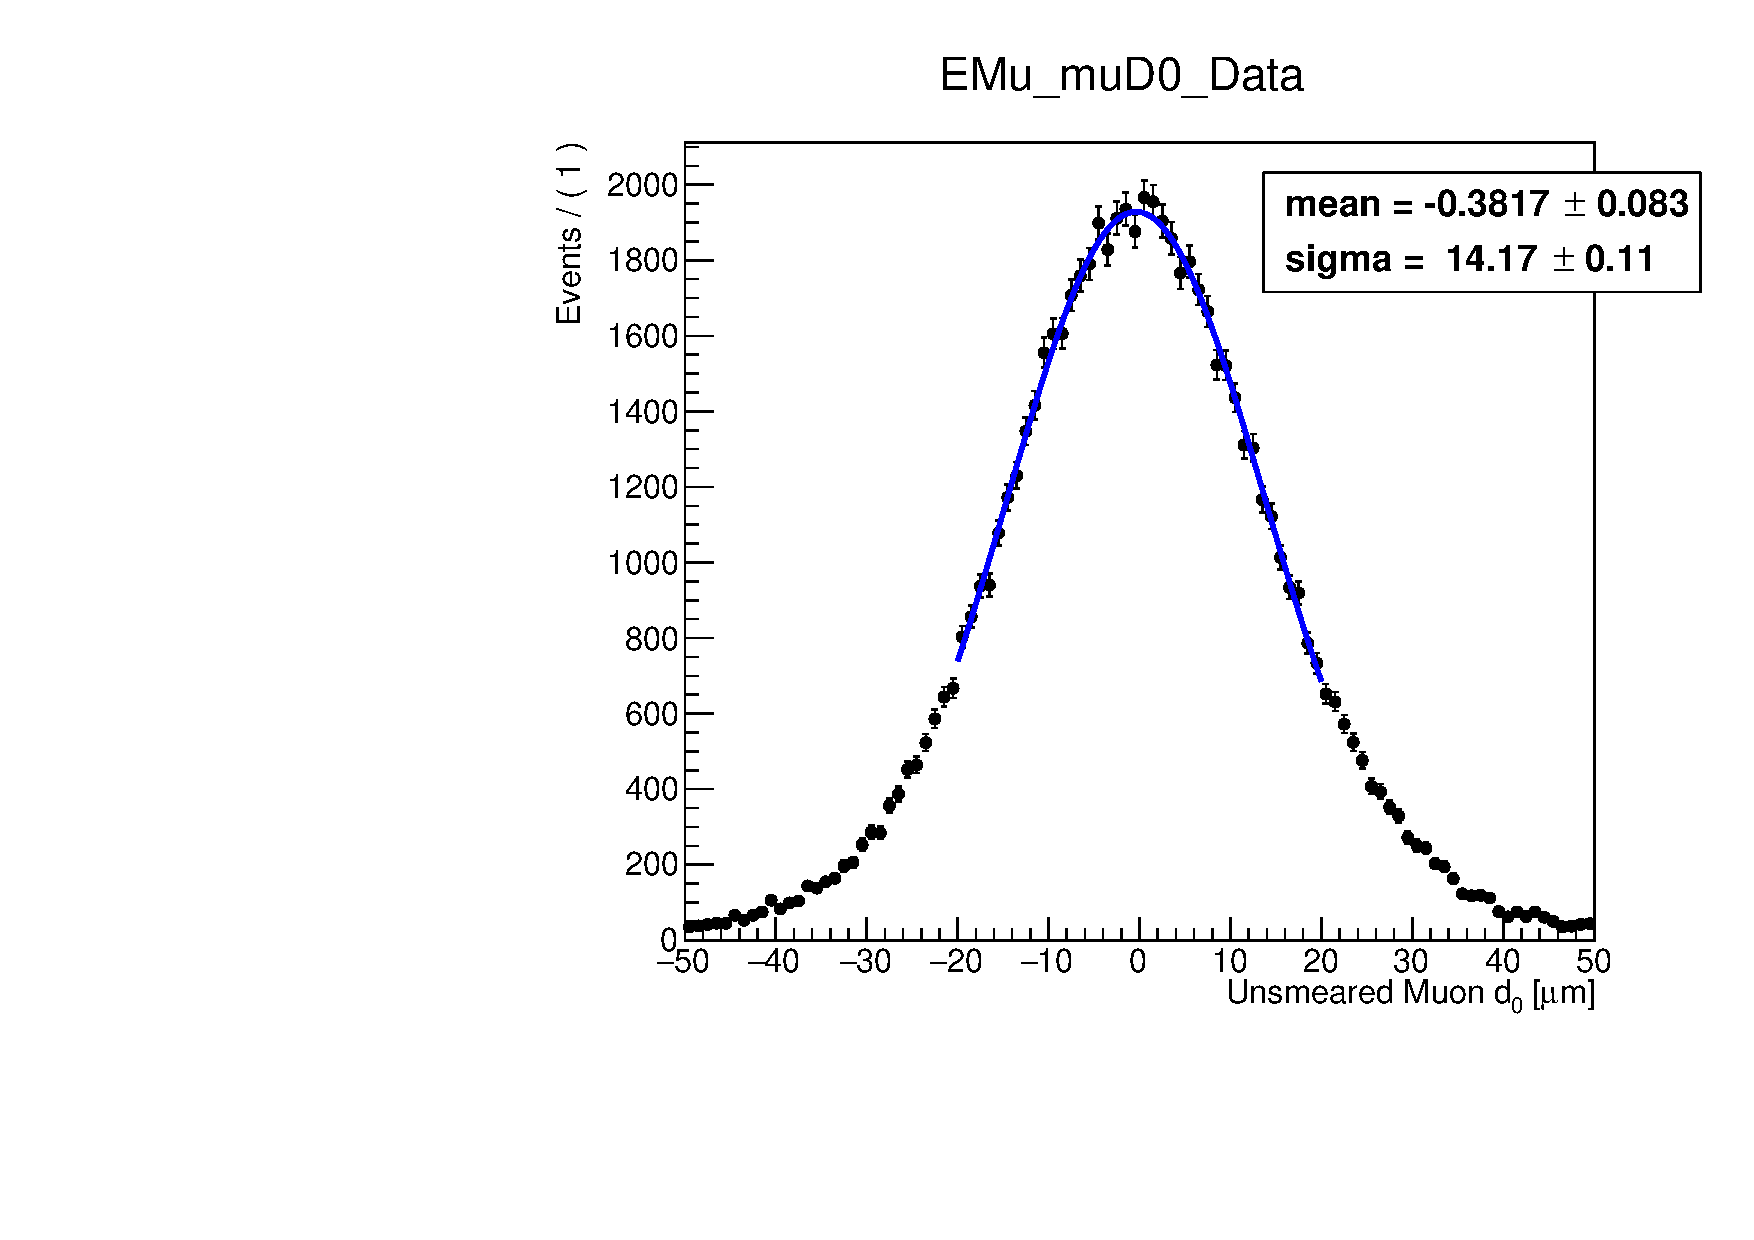
\includegraphics[scale=0.3]{figures/corrections/d0_smearing/emu_2017/gaussian_fit_EMu_muD0_Data.pdf} 
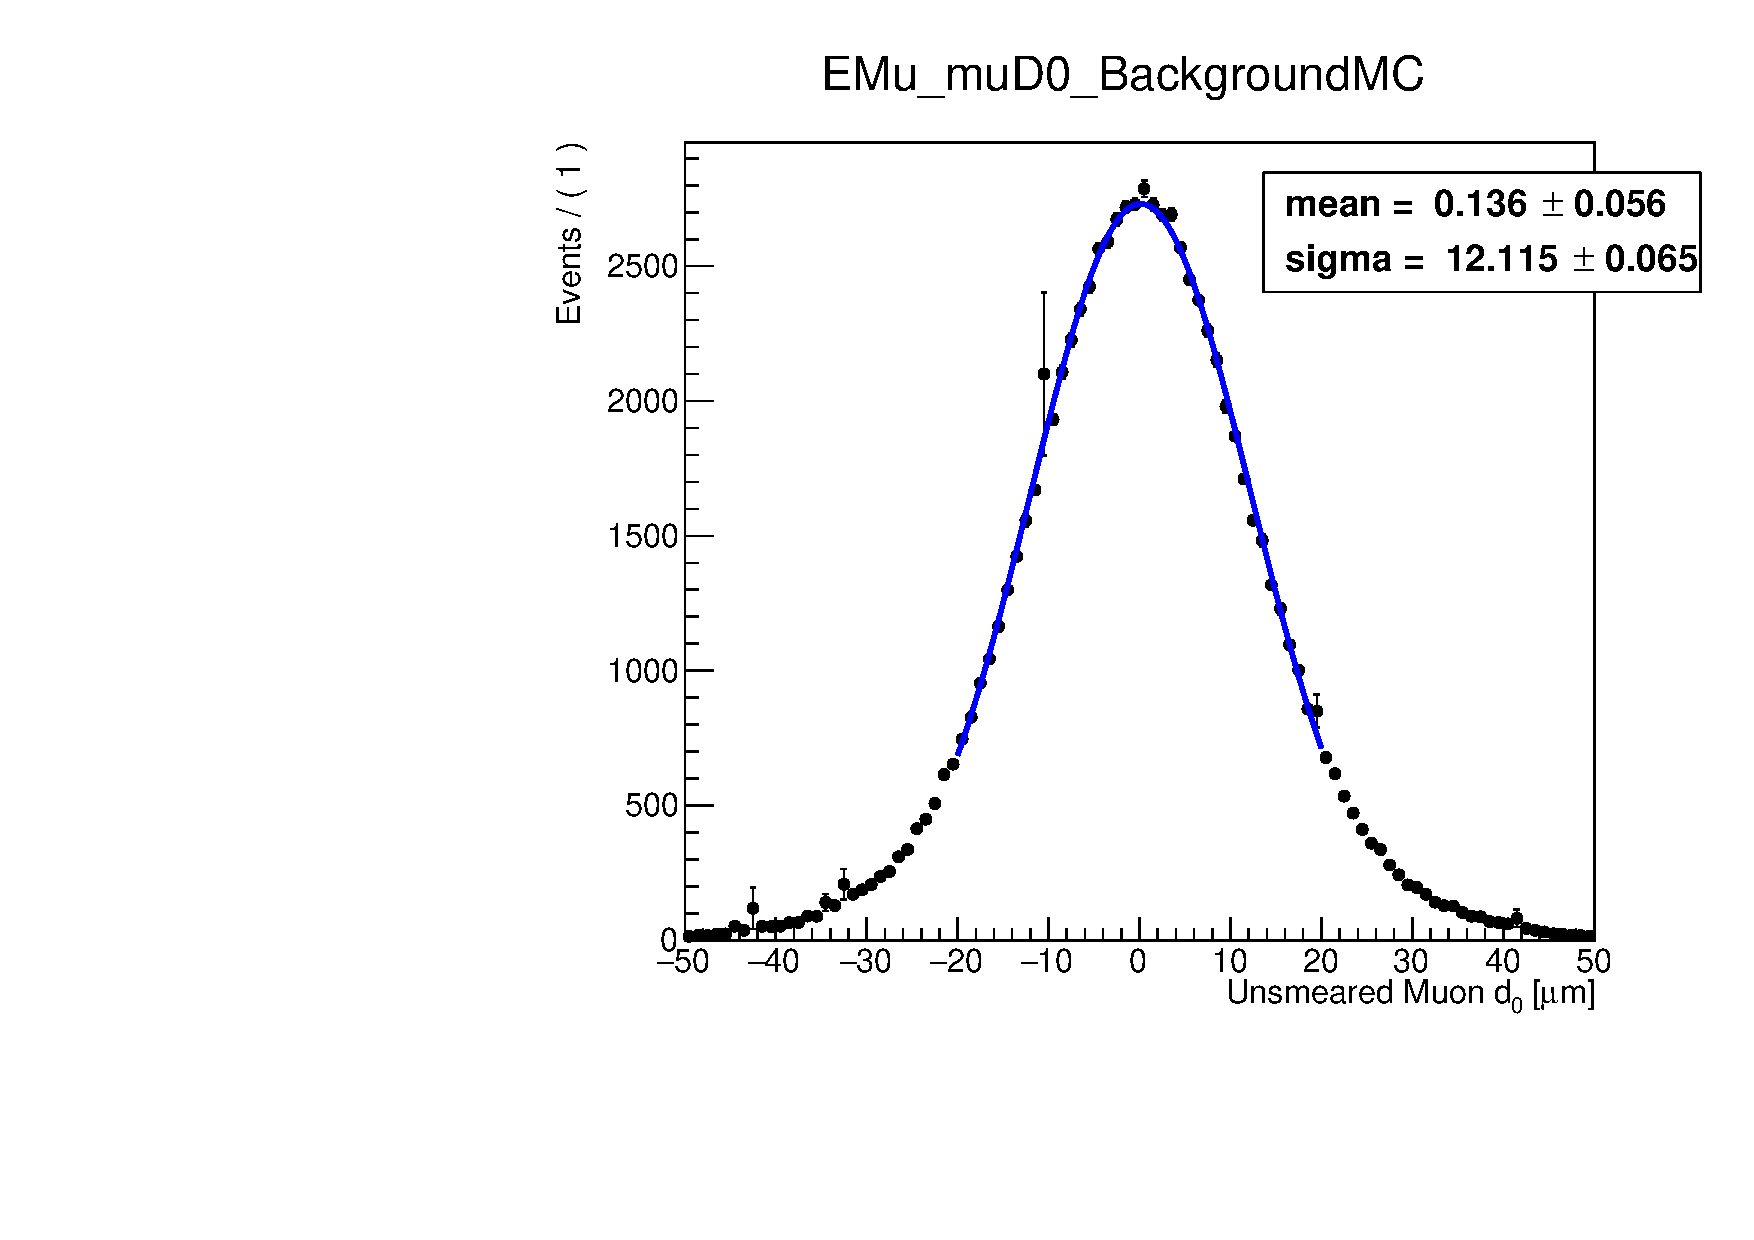
\includegraphics[scale=0.3]{figures/corrections/d0_smearing/emu_2017/gaussian_fit_EMu_muD0_BackgroundMC.pdf}
\caption{The lepton $d_0$ distributions with Gaussian fits in data (left) and background simulation (right) for electrons (upper) and muons (lower) in the 2017 $\Pe\Pgm$ prompt control region. The widths of the Gaussian fits are used to determine the width of the Gaussian distribution used to smear the $d_0$.}
\label{gaussian_fits_2017}
\end{figure}

\begin{figure}[hbtp]
\centering
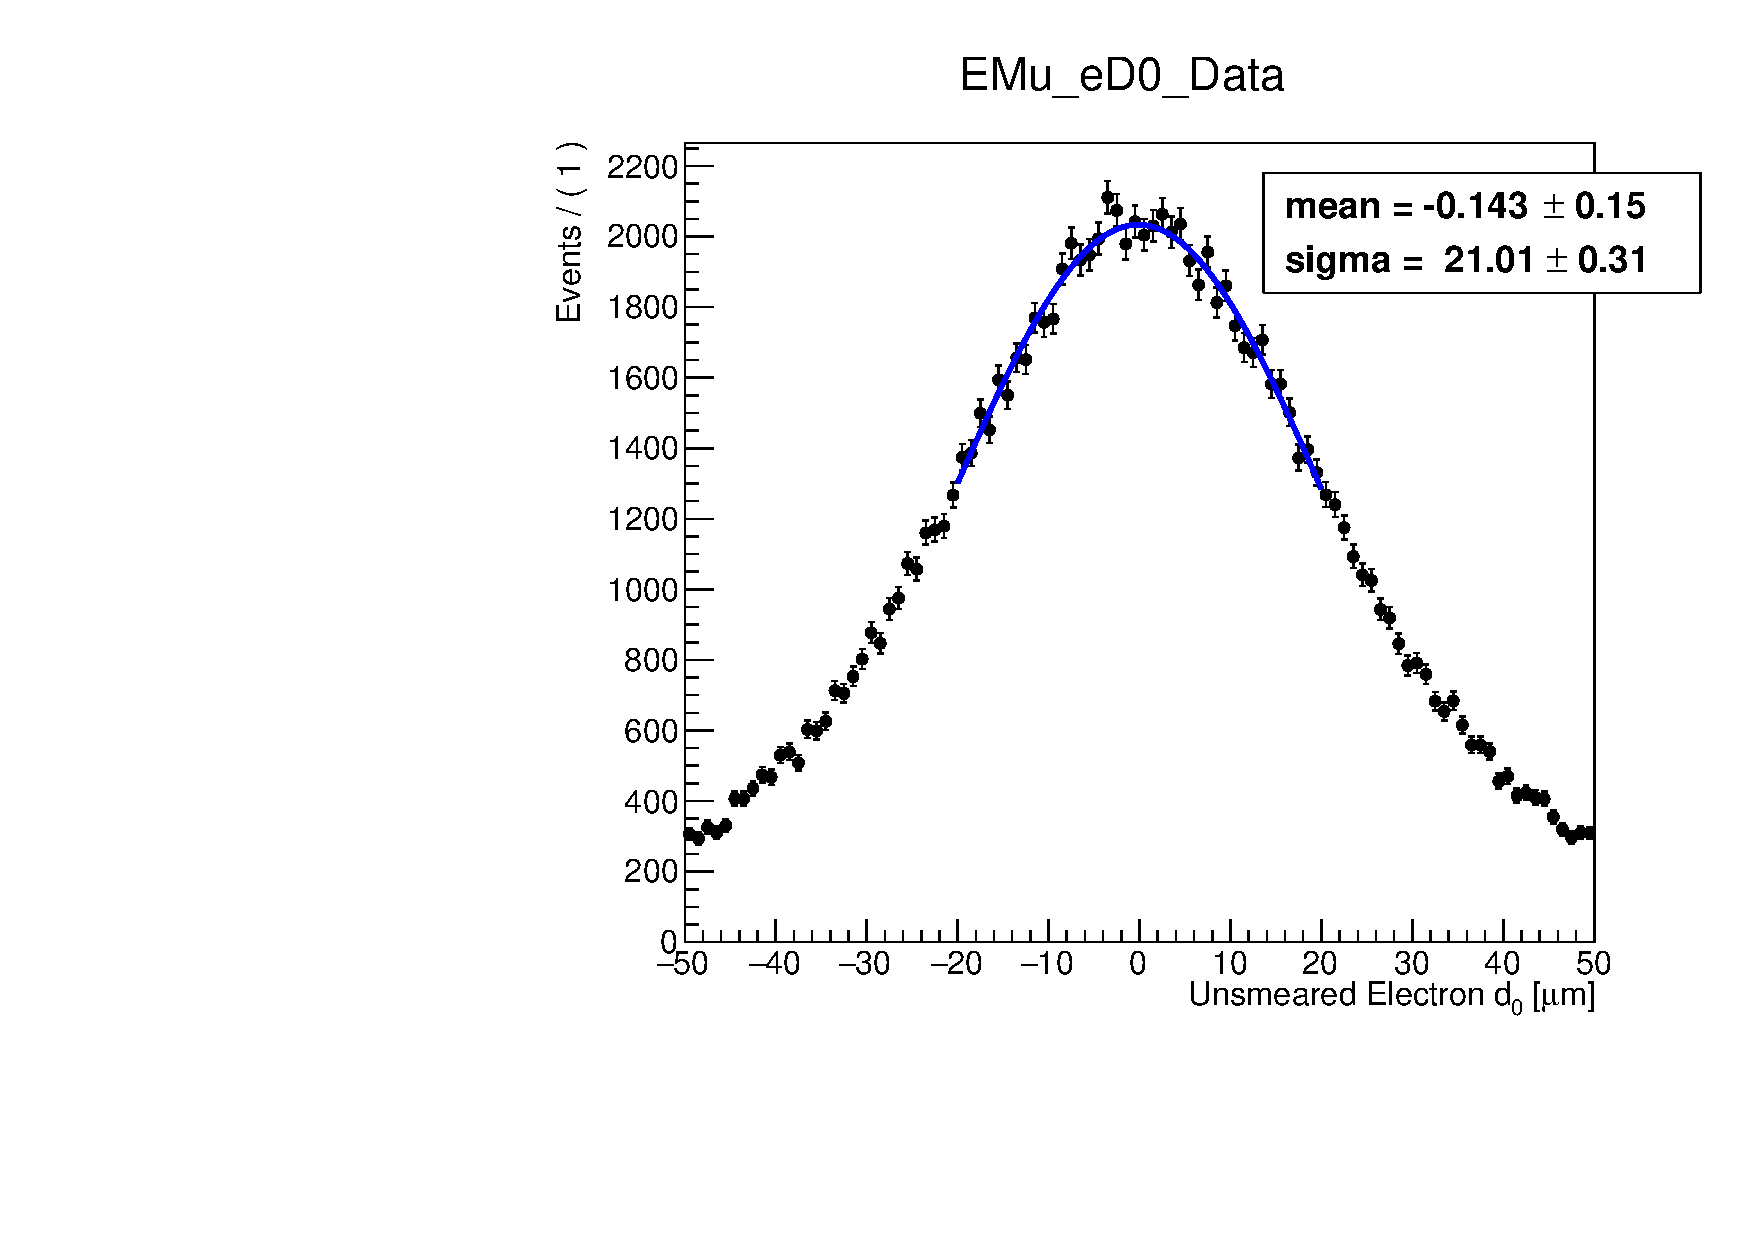
\includegraphics[scale=0.3]{figures/corrections/d0_smearing/emu_2018/gaussian_fit_EMu_eD0_Data.pdf}
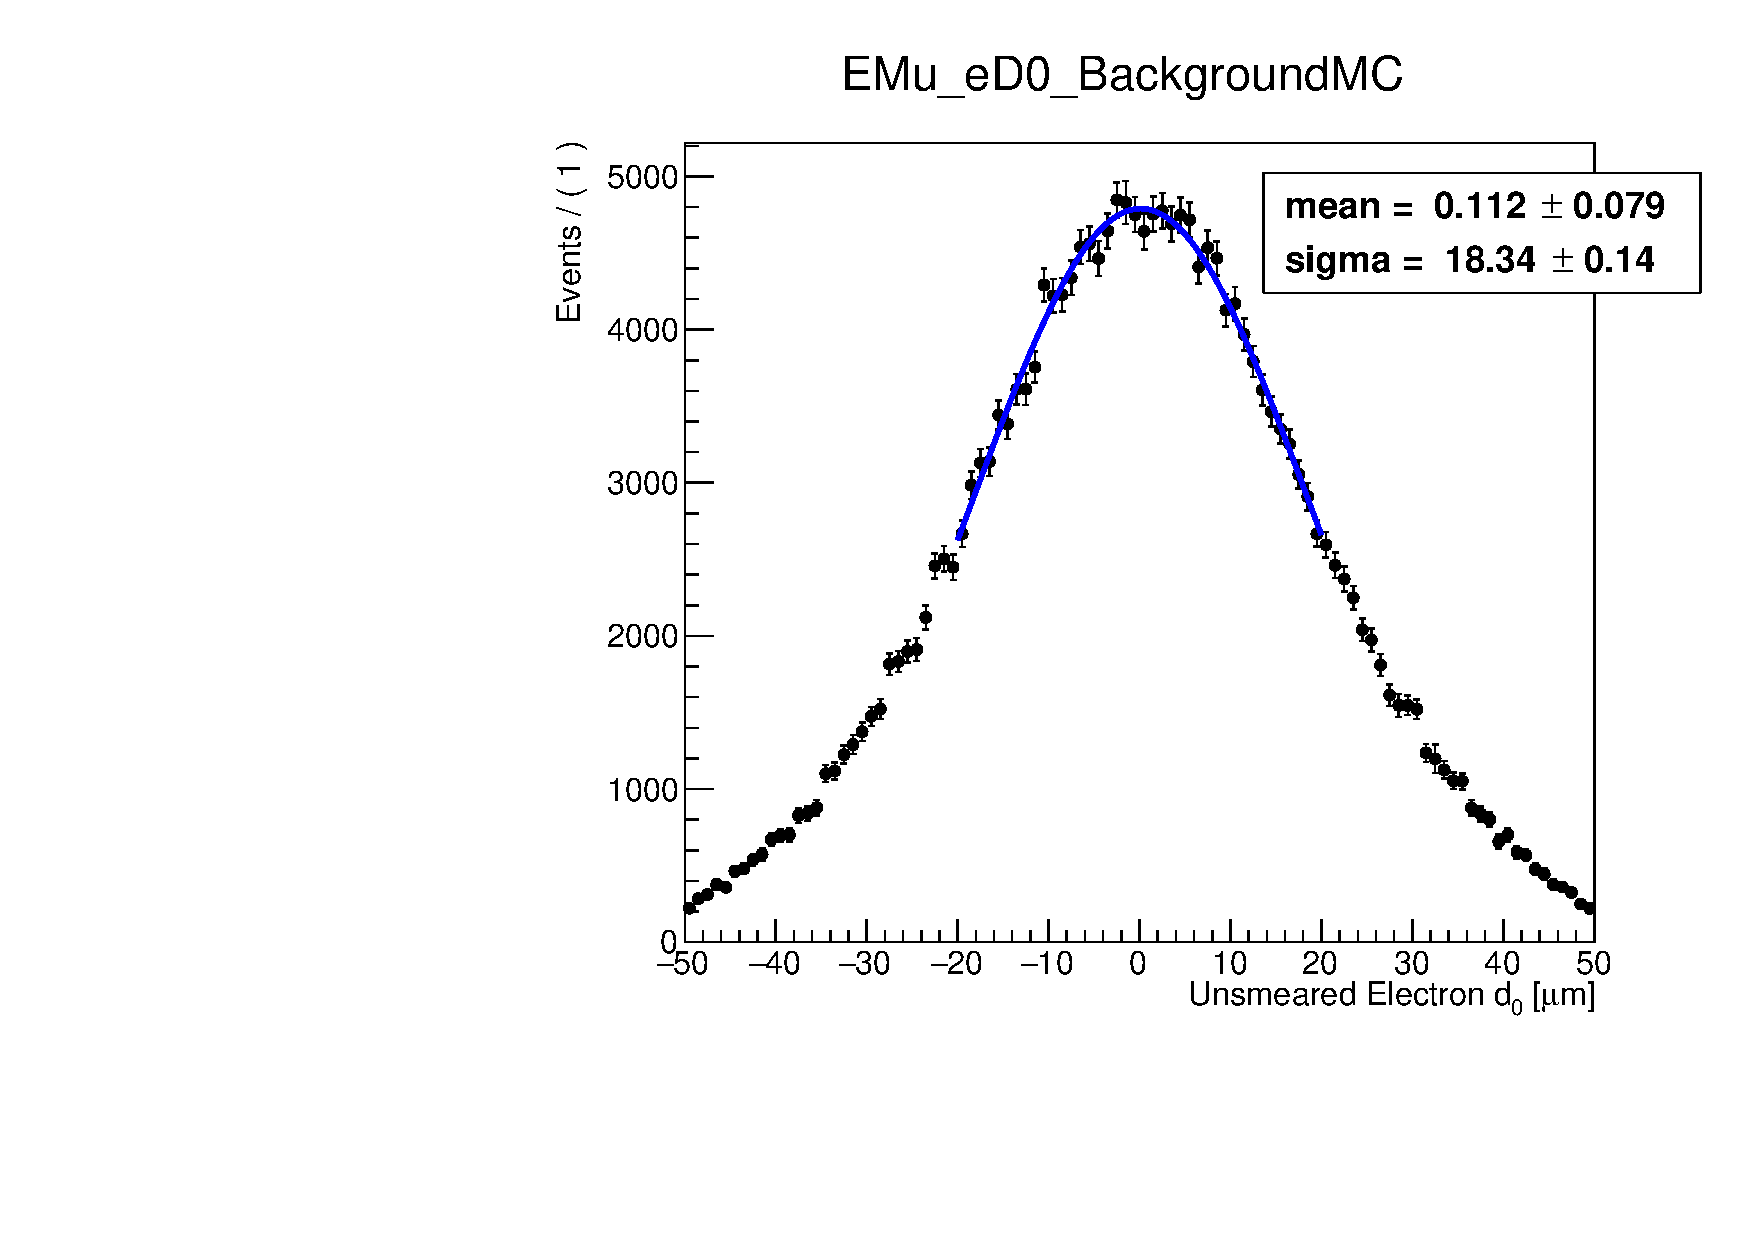
\includegraphics[scale=0.3]{figures/corrections/d0_smearing/emu_2018/gaussian_fit_EMu_eD0_BackgroundMC.pdf}
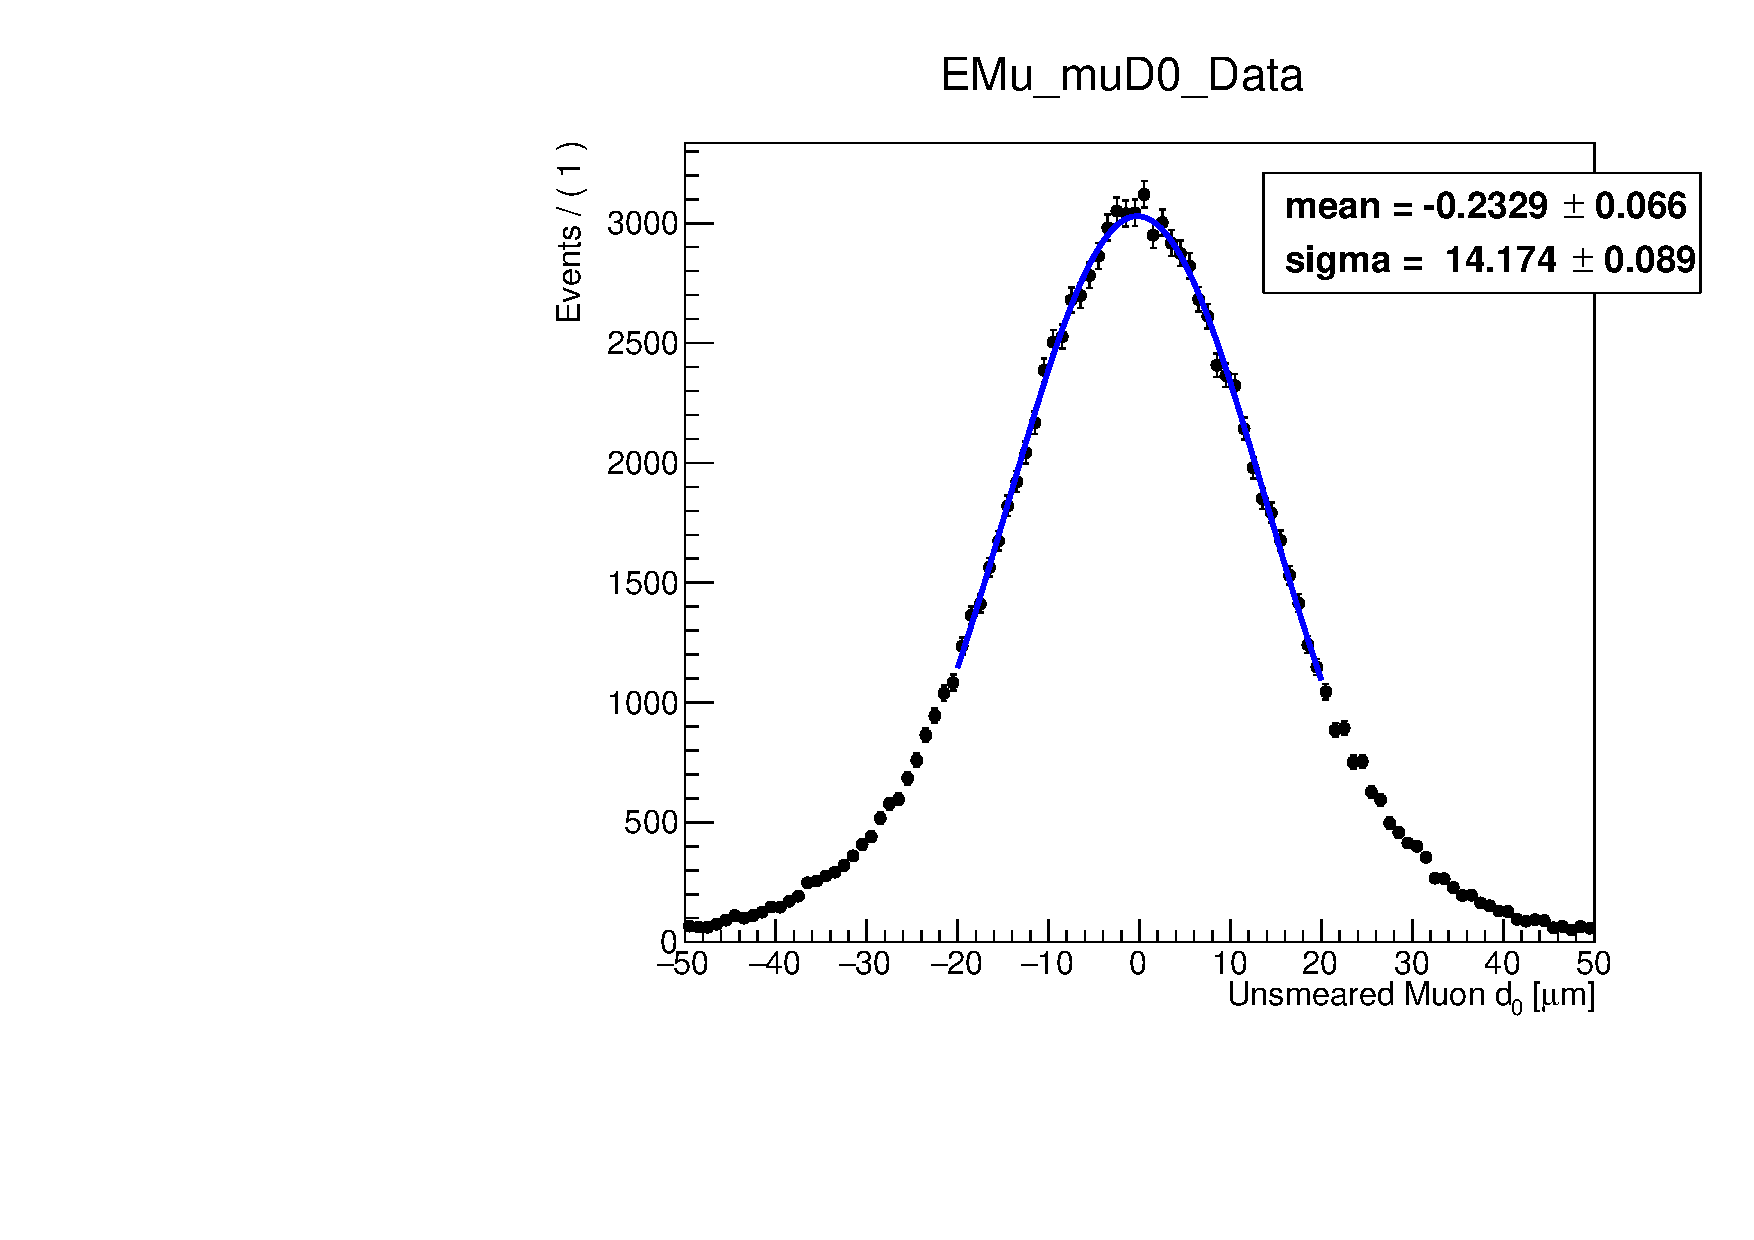
\includegraphics[scale=0.3]{figures/corrections/d0_smearing/emu_2018/gaussian_fit_EMu_muD0_Data.pdf} 
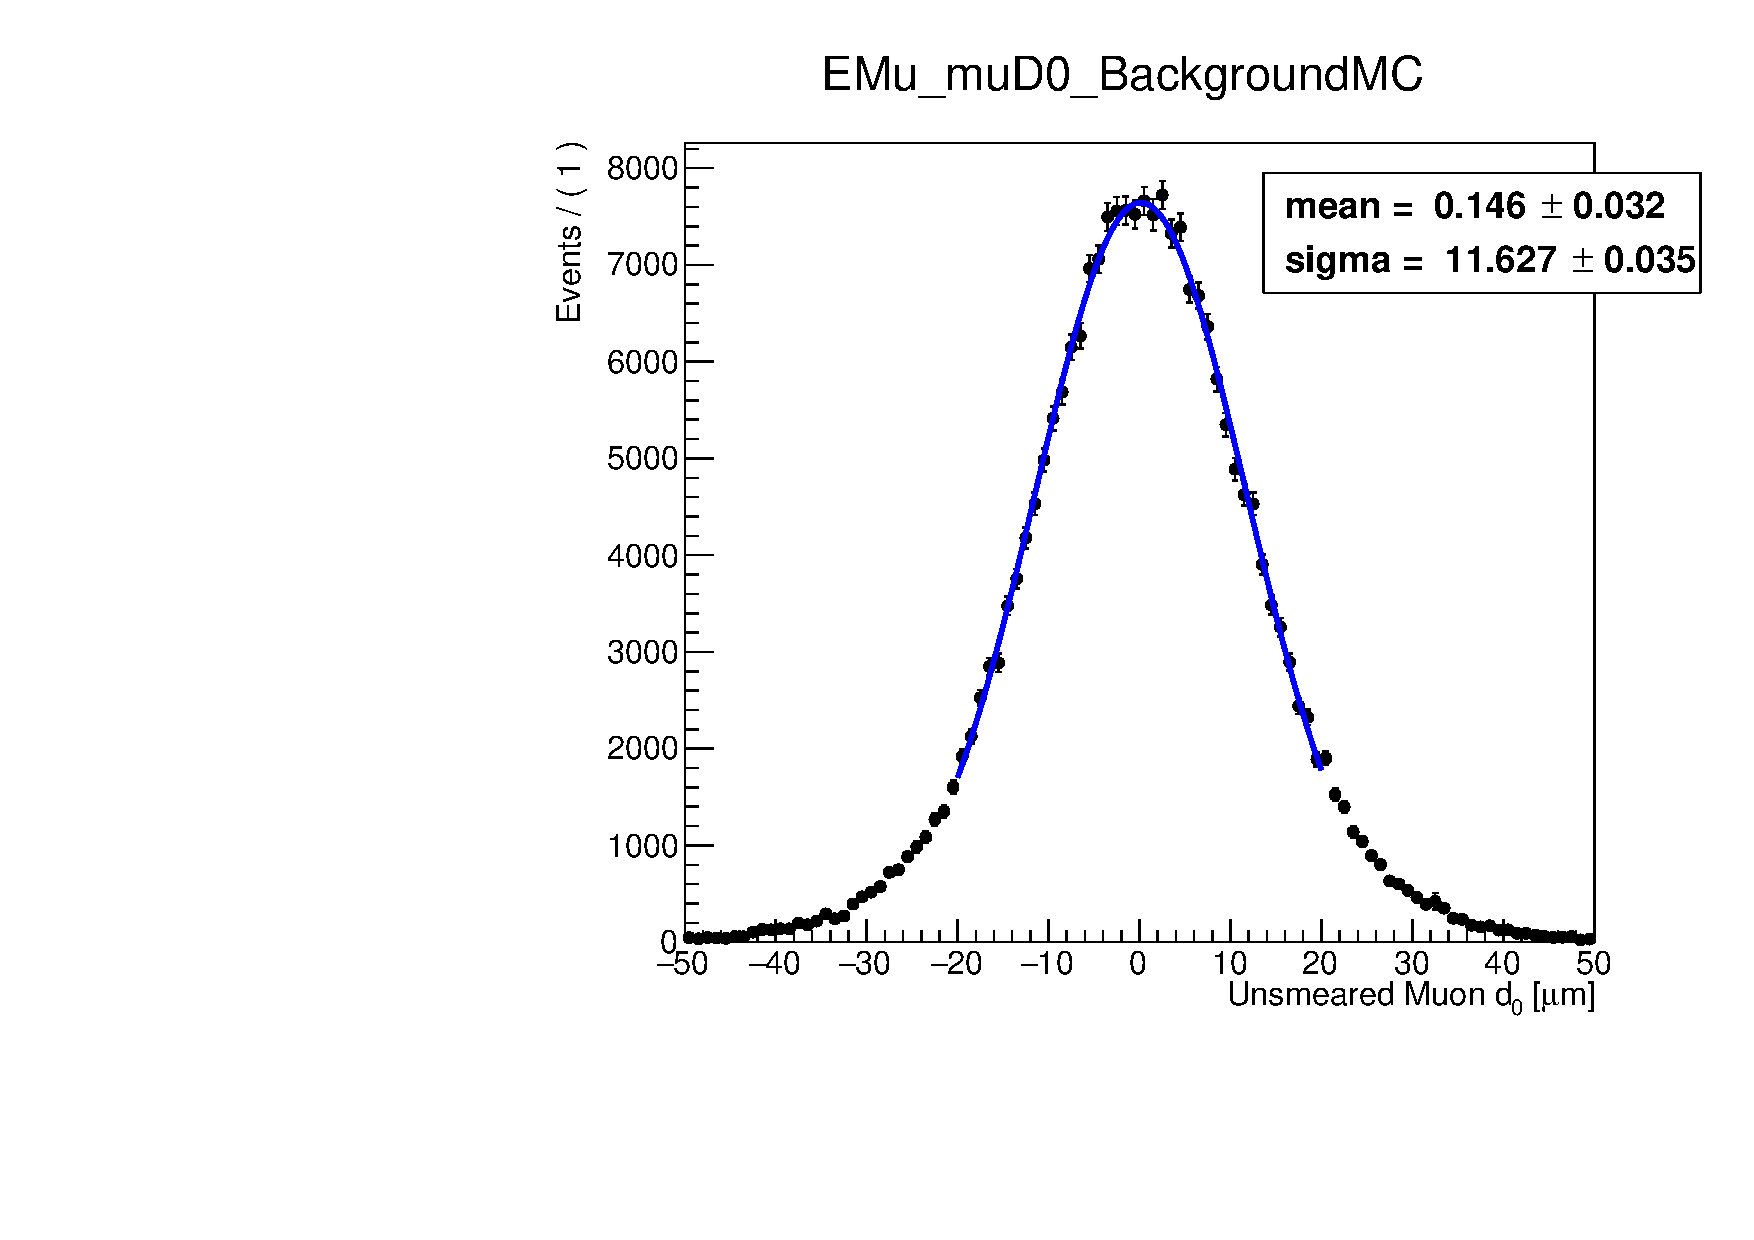
\includegraphics[scale=0.3]{figures/corrections/d0_smearing/emu_2018/gaussian_fit_EMu_muD0_BackgroundMC.pdf}
\caption{The lepton $d_0$ distributions with Gaussian fits in data (left) and background (right) for electrons (upper) and muons (lower) in the 2018 $\Pe\Pgm$ prompt control region. The widths of the Gaussian fits are used to determine the width of the Gaussian distribution used to smear the $d_0$.}
\label{gaussian_fits_2018}
\end{figure}
\begin{table}
\noindent \centering{}
\topcaption{The average $\sigma_{align}$ for electrons and muons, for the 2017 and 2018 analyses.}
\label{sigma_align}
\begin{tabular}{l|ccc}
\hline
          & 2017      & 2018\\
\hline
Electrons & $14.75\pm0.36\mum$ & $9.18\pm0.41\mum$\\
Muons     & $7.57\pm0.12\mum$  & $8.11\pm0.08\mum$\\
\hline
\end{tabular}
\end{table}
\begin{figure}
\centering
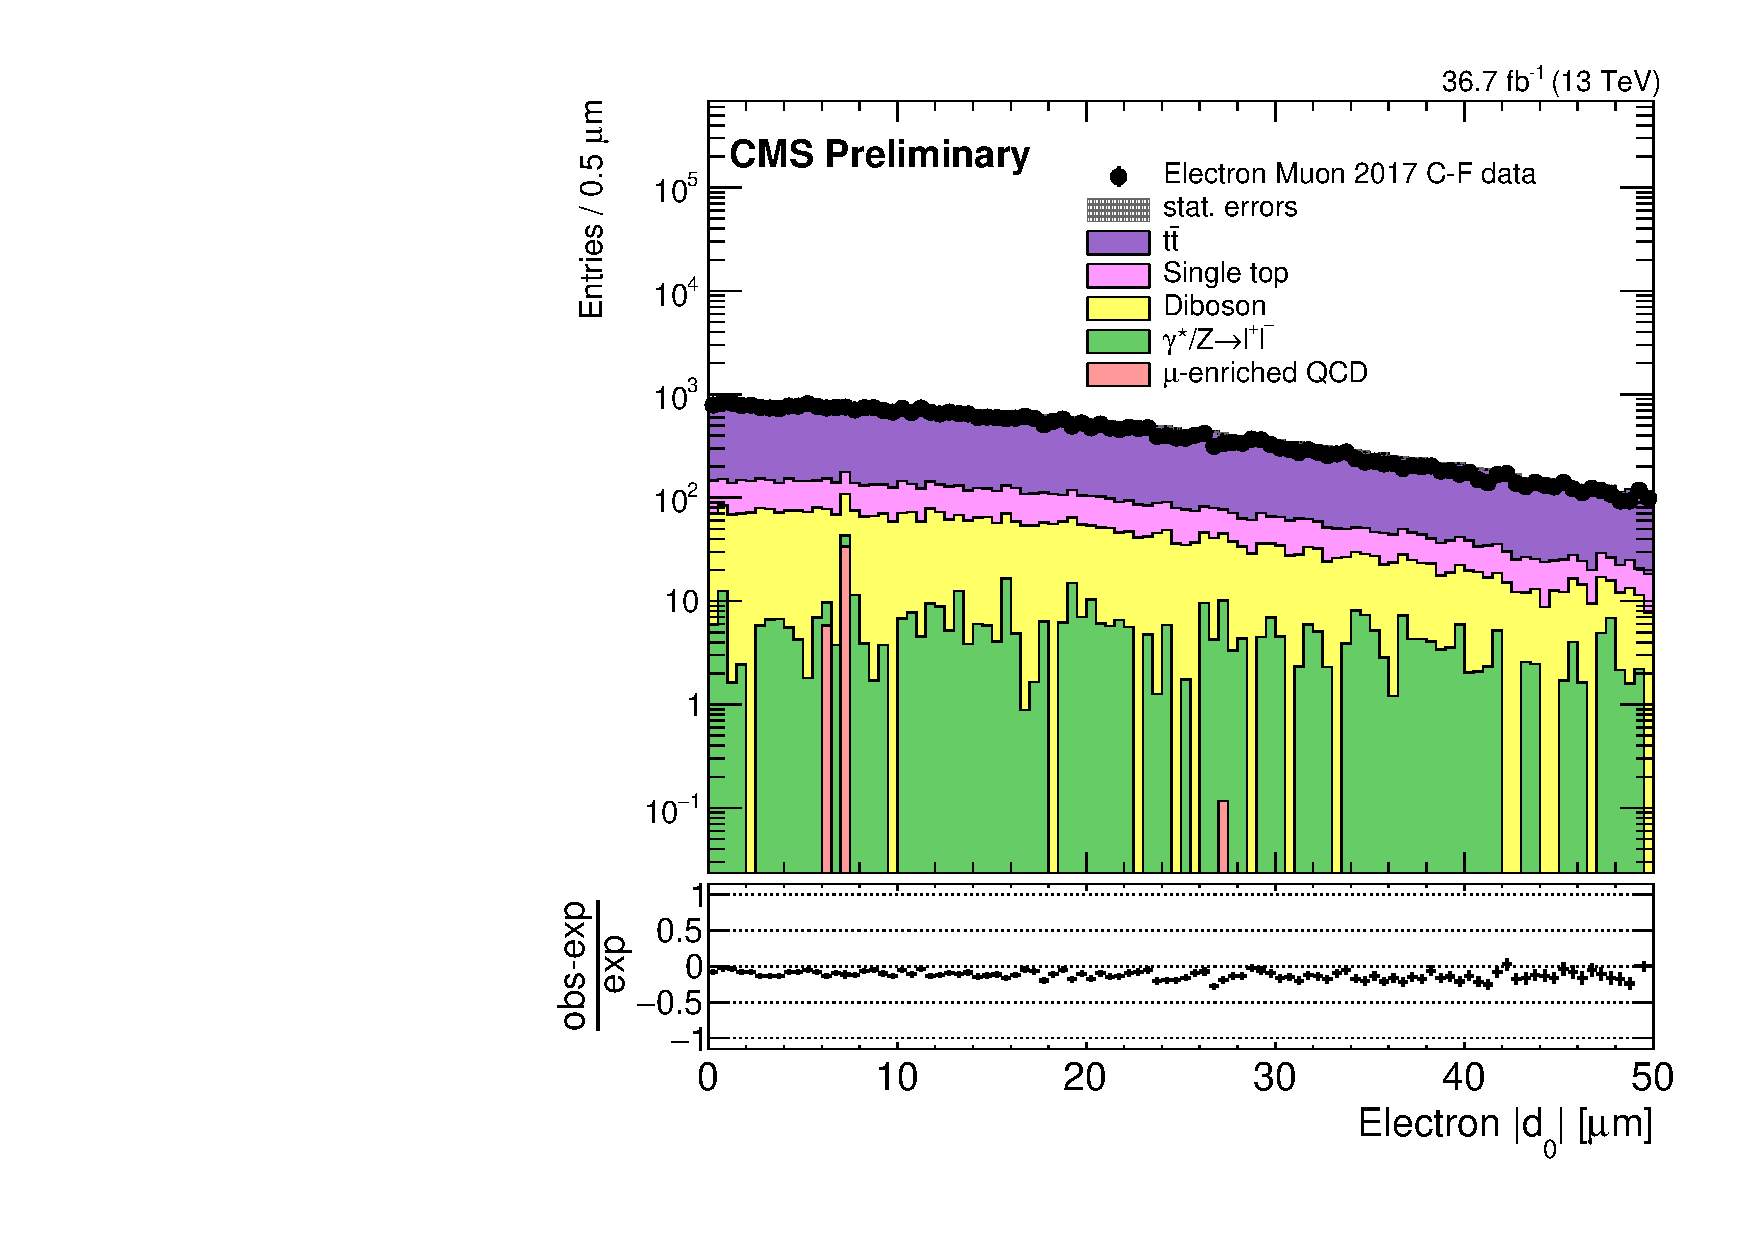
\includegraphics[width=0.4\textwidth]{figures/corrections/d0_smearing/emu_2017/electronAbsD0_50um.pdf} 
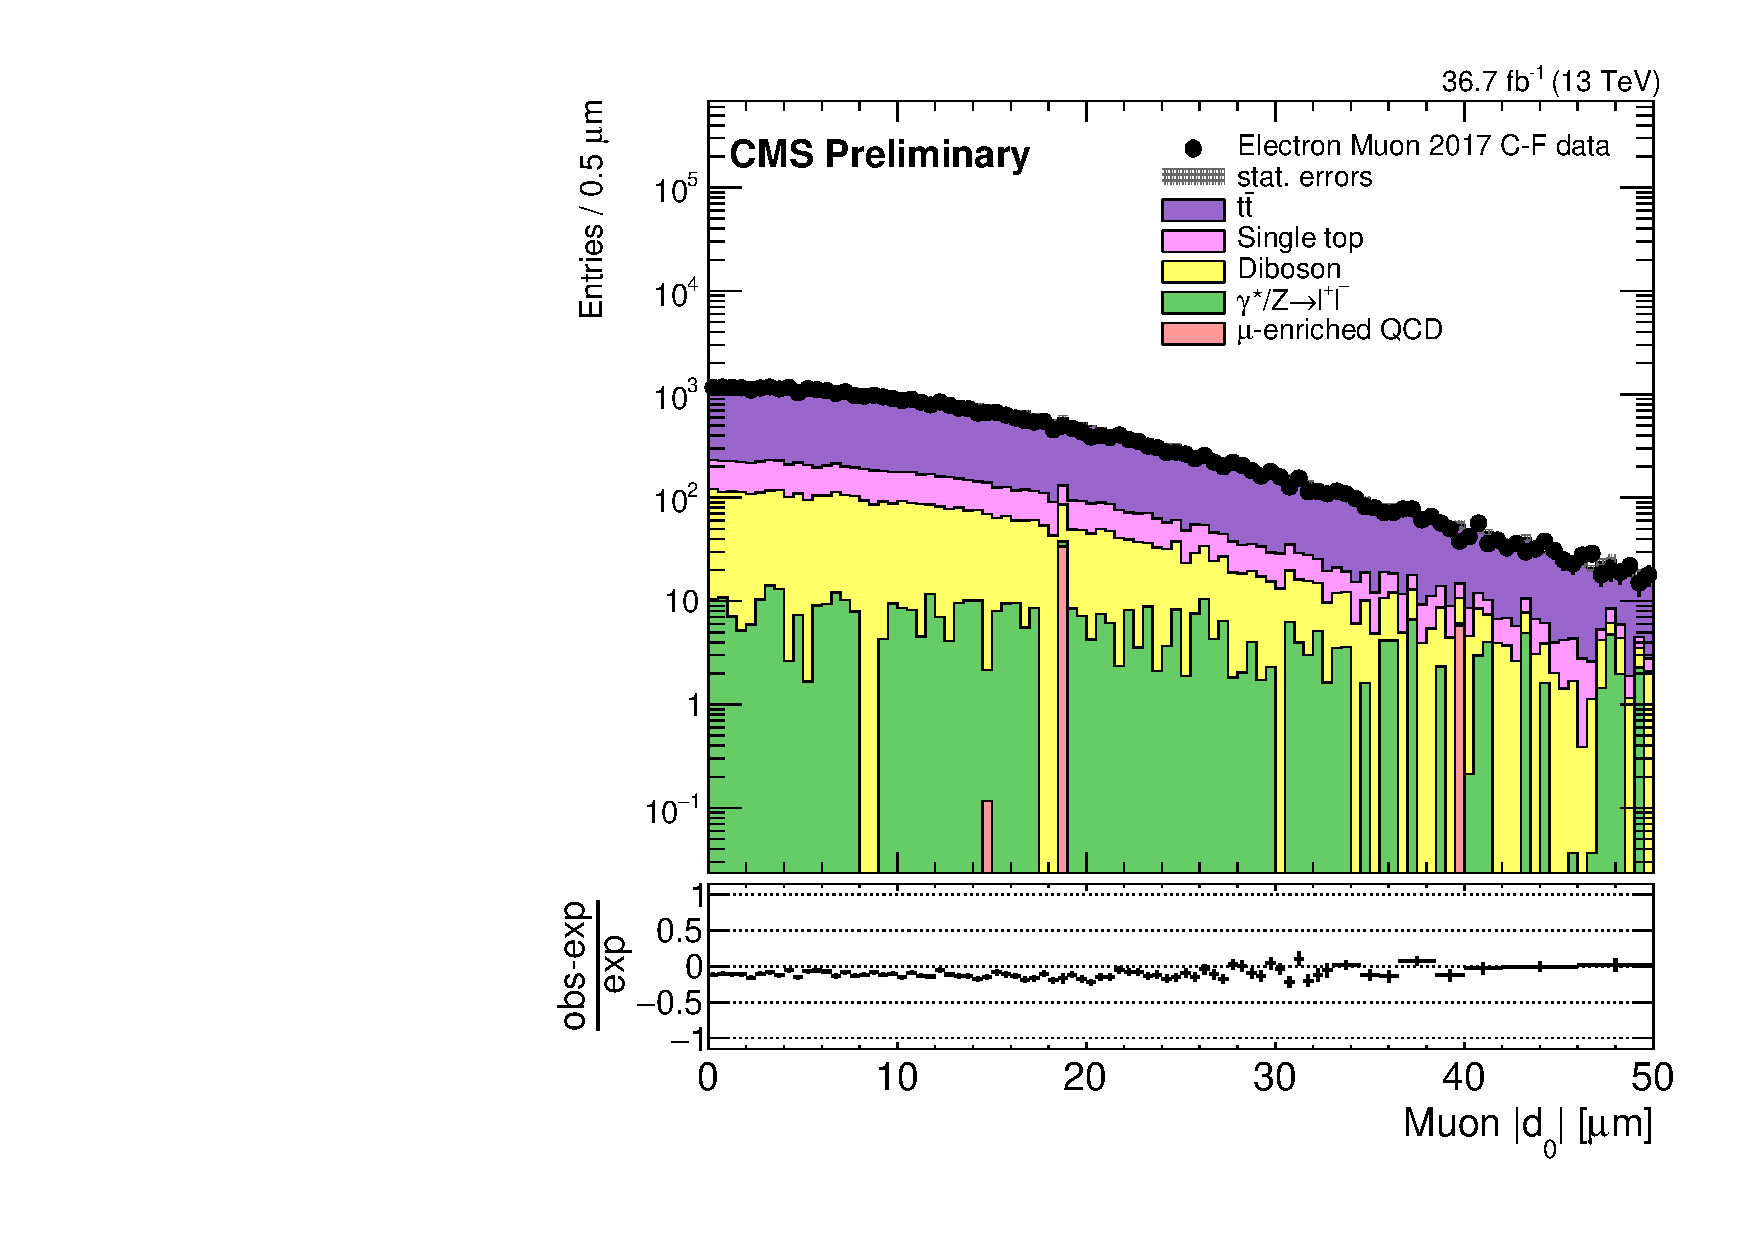
\includegraphics[width=0.4\textwidth]{figures/corrections/d0_smearing/emu_2017/muonAbsD0_50um.pdf}
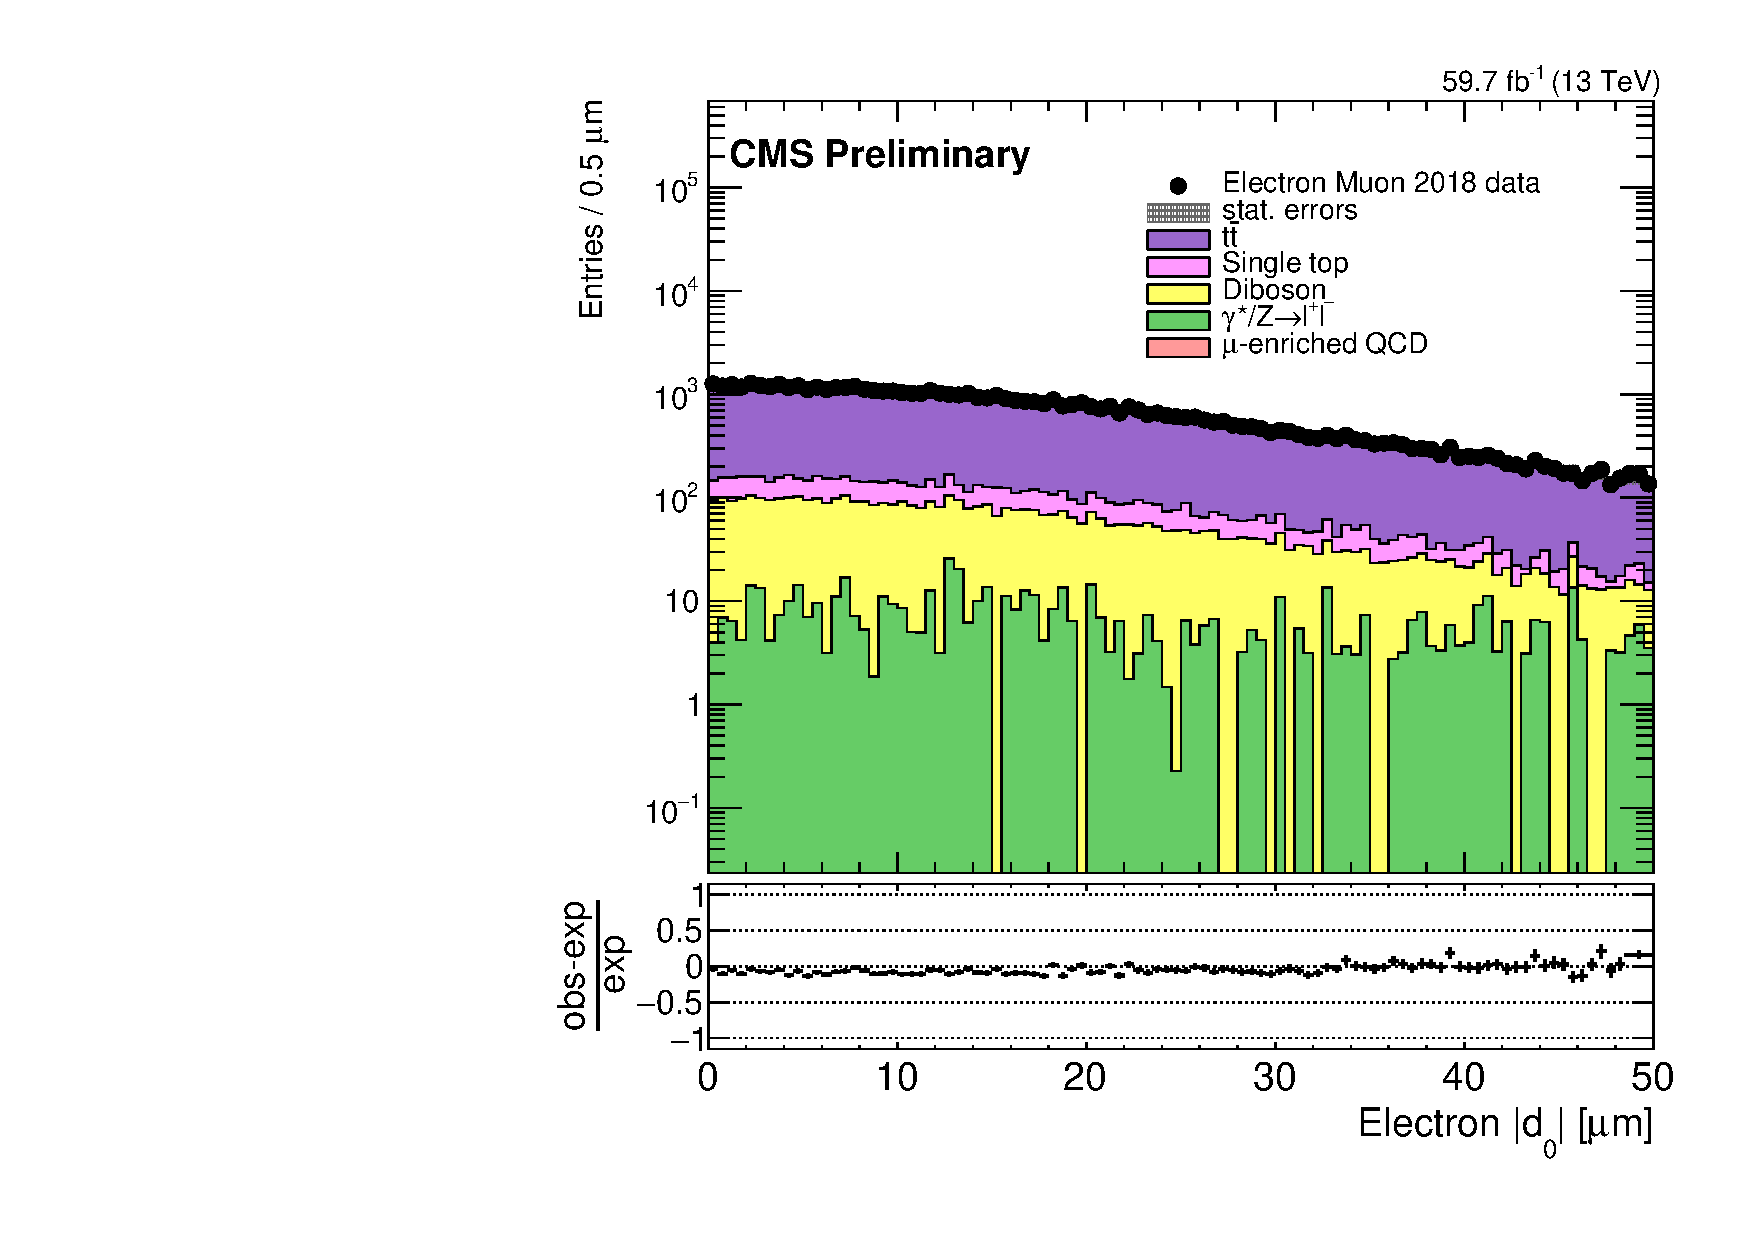
\includegraphics[width=0.4\textwidth]{figures/corrections/d0_smearing/emu_2018/electronAbsD0_50um.pdf} 
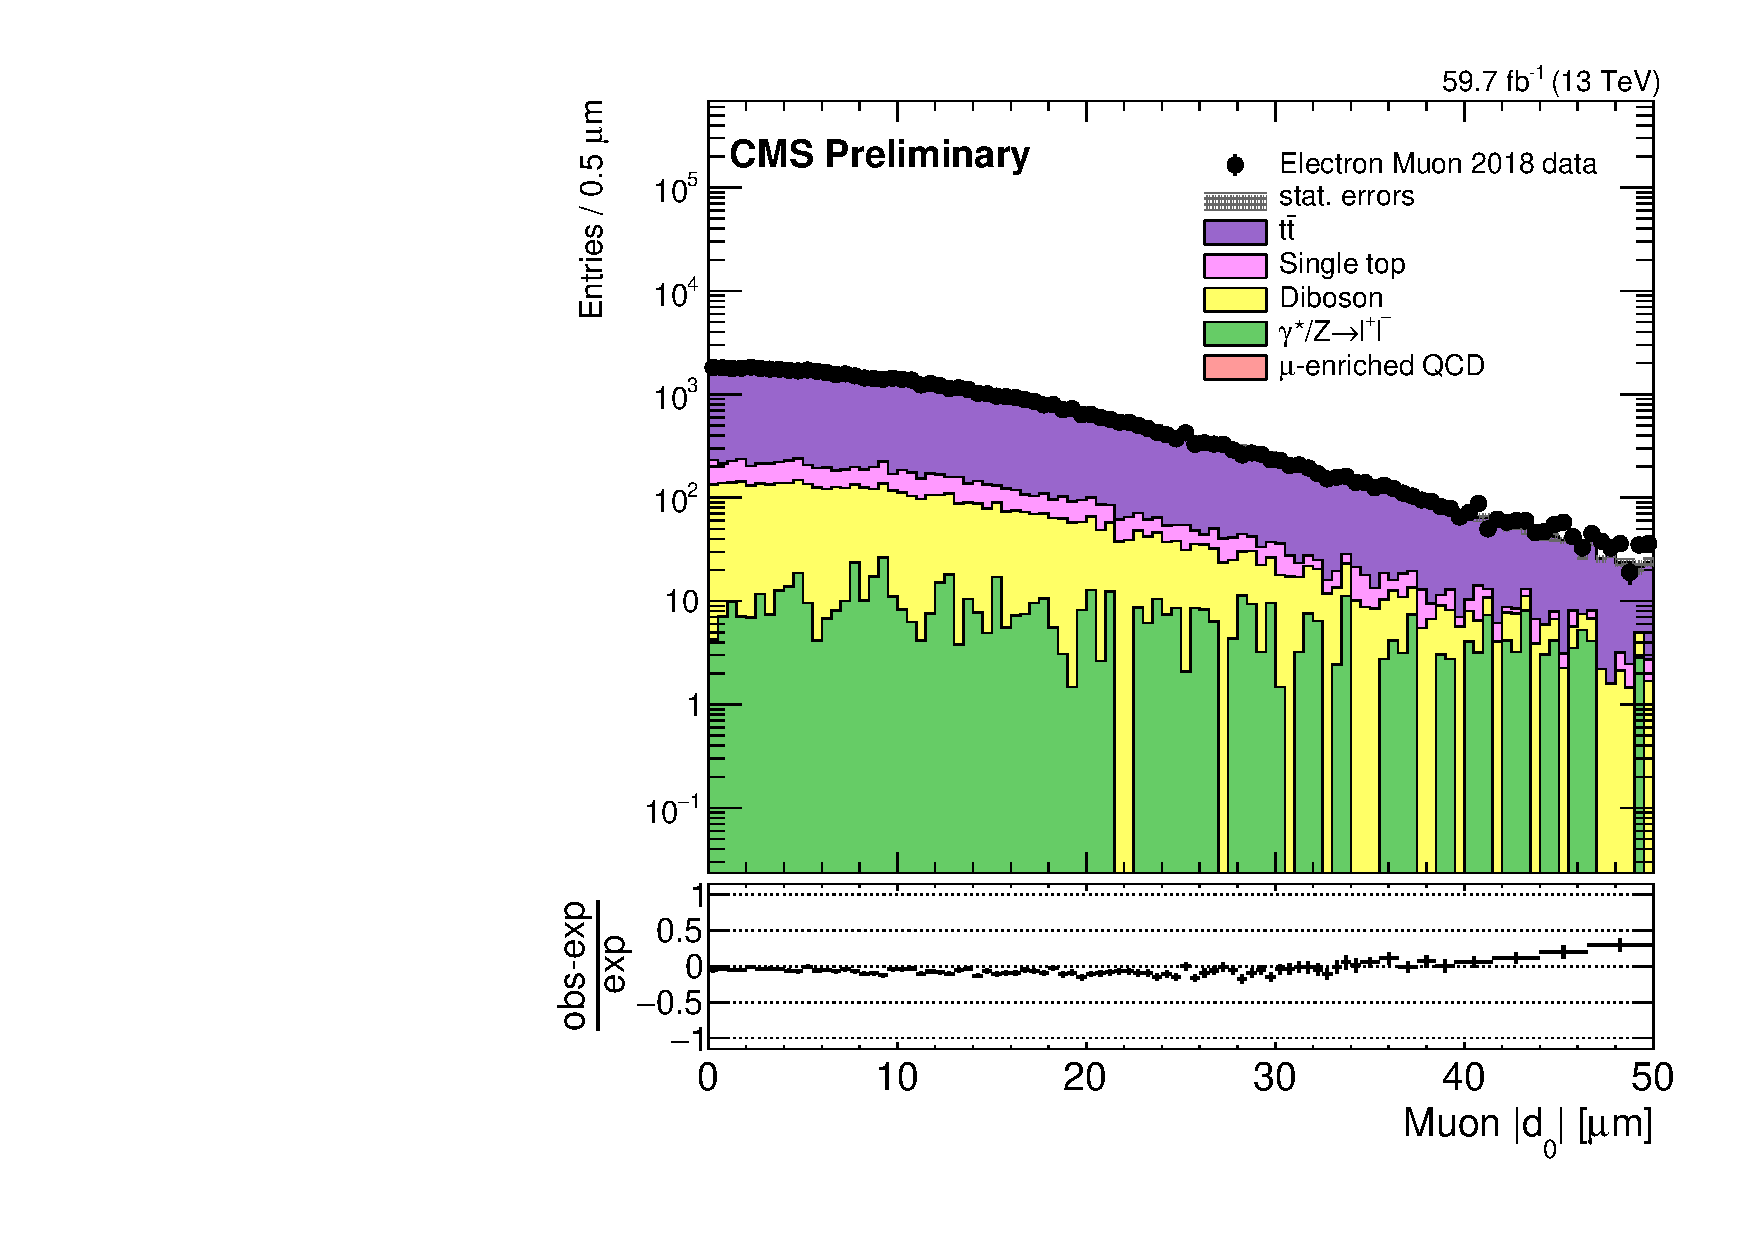
\includegraphics[width=0.4\textwidth]{figures/corrections/d0_smearing/emu_2018/muonAbsD0_50um.pdf}
\caption{The corrected lepton \ad distributions in the $\Pe\Pgm$ prompt control region, for electrons (left) and muons (right), for 2017 data and simulation (top), and 2018 data and simulation (bottom). The rightmost bin in each plot
contains the overflow entries.}
\label{corrected_d0}
\end{figure}

This $d_0$ smearing has a minimal effect on the final result because the width of the Gaussian distribution from which the smearing values are drawn is small relative to the size of the signal region bins, but understanding the source of the poor agreement between data and simulation was important to validate our understanding of the SM background.

\subsection{Trigger efficiency}
\label{trigger_eff}
We also apply scale factors to the simulated background and signal events to correct for differences in trigger efficiency between data and simulation. To measure the trigger efficiency, we first require that events pass an OR of several unprescaled \ptmiss triggers (see Table~\ref{triggers_met}) and the preselection criteria with the lepton \pt requirement excluded. The \ptmiss triggers provide a sample of dilepton events that is unbiased with respect to the main triggers used in the analysis, and excluding the lepton \pt requirement allows us to study the trigger efficiency as a function of lepton \pt. In the $\Pe\Pgm$ channel, the electron (muon) \pt is required to be greater than 50\GeV when plotting against the muon (electron) \pt to disentangle the effect from the other leg of the muon-photon trigger. Data events are taken from the \texttt{MET} primary dataset (which contains events that pass \ptmiss trigger) and simulated background events are taken from $\ttbar$\fxnote{define?} simulation for the $\Pe\Pgm$ channel and Drell-Yan simulation for the same-flavor channels. To calculate the efficiency, we divide the lepton \pt distribution in events that pass the standard analysis triggers in addition to the OR of the \ptmiss triggers and the preselection by the lepton \pt distribution in events that pass the OR of the \ptmiss triggers and the preselection. We then compute the scale factor as the ratio of the efficiency in data to the efficiency in simulation in the plateau of the efficiency distribution.\fxnote{add plots}

\begin{table}
\noindent \centering{}
\topcaption{The unprescaled MET triggers used to create an orthogonal data sample for the trigger efficiency calculation.}
\label{triggers_met}
\begin{tabular}{l}
\hline
\textbf{2016}    \\
HLT\_MET200 \\
HLT\_MonoCentralPFJet80\_PFMETNoMu110\_PFMHTNoMu110\_IDTight \\
HLT\_PFMET120\_PFMHT120\_IDTight \\
HLT\_PFMET170\_HBHECleaned \\
HLT\_PFMET300 \\
HLT\_PFMETNoMu120\_PFMHTNoMu120\_IDTight \\
\end{tabular}
\bigskip

\begin{tabular}{l}
\textbf{2017}    \\
HLT\_CaloMET350\_HBHECleaned \\
HLT\_MonoCentralPFJet80\_PFMETNoMu120\_PFMHTNoMu120\_IDTight \\
HLT\_PFMET120\_PFMHT120\_IDTight \\
HLT\_PFMET250\_HBHECleaned \\
HLT\_PFMETNoMu120\_PFMHTNoMu120\_IDTight \\
\end{tabular}

\bigskip

\begin{tabular}{l}
\textbf{2018}    \\
HLT\_CaloMET350\_HBHECleaned \\
HLT\_MonoCentralPFJet80\_PFMETNoMu120\_PFMHTNoMu120\_IDTight \\
HLT\_PFMET120\_PFMHT120\_IDTight \\
HLT\_PFMET200\_HBHE\_BeamHaloCleaned \\
HLT\_PFMET250\_HBHECleaned \\
HLT\_PFMETNoMu120\_PFMHTNoMu120\_IDTight \\
\hline
\end{tabular}
\end{table}


\pagebreak